% ═══════════════════════════════════════════════════════════════════════════════
% Protein Surface Classification on SHREC 25: A Hierarchical GNN Study
% ═══════════════════════════════════════════════════════════════════════════════
\documentclass[11pt,a4paper]{article}

% ── Packages ──────────────────────────────────────────────────────────────────
\usepackage[a4paper, margin=2.5cm]{geometry}
\usepackage{graphicx}
\usepackage{booktabs}
\usepackage{amsmath}
\usepackage{amssymb}
\usepackage{subcaption}
\usepackage{float}
\usepackage{xcolor}
\usepackage[hidelinks, colorlinks=true, linkcolor=blue!60!black,
            citecolor=green!50!black, urlcolor=blue]{hyperref}
\usepackage{microtype}
\usepackage{parskip}
\usepackage[T1]{fontenc}
\usepackage{lmodern}

% ── Title ─────────────────────────────────────────────────────────────────────
\title{%
  \textbf{Protein Surface Classification on SHREC\,25}\\[0.5ex]
  \large A Comprehensive Study: Data Pipeline, Statistical Analysis,\\
  Hierarchical GNN Architecture, and Feature Ablations
}
\author{%
  Protein Classification Study\\[0.3ex]
  \small Based on SHREC\,25 benchmark data
}
\date{June 2026}

% ─────────────────────────────────────────────────────────────────────────────
\begin{document}
\maketitle
\tableofcontents
\newpage

% ─────────────────────────────────────────────────────────────────────────────
% ─────────────────────────────────────────────────────────────────
\section{Introduction}
\label{sec:intro}
% ─────────────────────────────────────────────────────────────────

Protein fold classification is a central problem in structural bioinformatics.
The three-dimensional surface shape of a protein, together with its
electrostatic potential field, encodes information about its biochemical
function and evolutionary family.
The SHREC\,25 Shape Retrieval Contest~\cite{shrec25} provides a benchmark that
casts fold recognition as a closed-world, 99-class classification task on
protein surface meshes, with a strongly class-imbalanced training set of
9\,244 proteins.

\paragraph{Why this problem is hard.}
Three structural challenges make SHREC\,25 particularly demanding:
\begin{enumerate}
  \item \textbf{Class imbalance.}
        The most frequent class (class\,8) has 2\,054 training examples while
        the rarest class has only 2 --- a 1\,027$\times$ ratio.
        Eleven classes have zero test proteins; evaluating macro-averaged F1
        over the 88 testable classes directly penalises poor recall on rare
        classes.

  \item \textbf{Near-inseparable class pairs.}
        Several protein families share highly similar surface geometry and
        electrostatics.
        The pair (class\,61, class\,90), for instance, is not separated by
        protein-level support-vector-machine classifiers on the provided surface
        features, even at full VTK resolution (balanced accuracy $\approx 0.56$).
        Section~\ref{sec:discussion:riconv2} shows this reflects the limits of
        single-scale descriptors rather than the data itself.

  \item \textbf{Surface-only feature budget.}
        The dataset provides only vertex positions, surface normals, and two
        scalar fields --- electrostatic potential (\textit{Potential}) and
        normal component of potential (\textit{NormalPotential}).
        Sequence information, volumetric electron density, and other richer
        representations are absent.
\end{enumerate}

\paragraph{Contributions.}
This report documents a complete end-to-end study with the following
contributions:
\begin{itemize}
  \item A preprocessing pipeline that converts VTK surface meshes into
        graph-learning-ready SSL graphs via farthest-point subsampling and
        k-nearest-neighbour edge construction
        (Section~\ref{sec:pipeline}).

  \item A statistical separability analysis at vertex level (Kolmogorov--Smirnov,
        Sliced Wasserstein), protein level (SVM on global statistics), and
        spatial level (Moran's~I autocorrelation) to characterise which
        features actually discriminate between classes
        (Section~\ref{sec:analysis}).

  \item A hierarchical graph neural network (\textit{HierGIN}) that stacks a
        node-level GIN over the 1\,000-node surface graph, a geodesic Voronoi
        patch pooling layer, and a patch-level GIN before global readout and
        classification (Section~\ref{sec:arch}).

  \item A rotation-invariant hierarchical architecture (\textit{RI-HierNet})
        that replaces the node-level GIN with four nested FPS + ball-query
        set-abstraction layers using point-pair invariant features,
        followed by a patch-level GIN over the 64 SA centroids
        (Section~\ref{sec:arch:rihiernet}).

  \item Systematic ablation of eight node-backbone types, five feature
        configurations, patch counts, hidden dimensions, and training
        regularisation choices (Section~\ref{sec:ablation}).

  \item A comparison with external methods (PointMamba~\cite{pointmamba},
        Mamba3D~\cite{mamba3d}) submitted to the SHREC\,25 contest, and an
        analysis of the theoretical performance ceiling imposed by the dataset
        structure (Section~\ref{sec:results}).
\end{itemize}

Our final RI-HierNet model achieves \textbf{accuracy\,=\,0.894} and
\textbf{weighted-F1\,=\,0.888}, a $+$2.7\,pp accuracy gain over the best
HierGIN-14D configuration (0.867) and a $+$4.1\,pp gain over the flat-GNN
baseline on accuracy.
HierGIN-14D remains the best model on macro-F1 (0.808 on the 88-class protocol),
as RI-HierNet is optimised for accuracy and weighted-F1 using unweighted
cross-entropy.
The confusion between class pairs (61,\,90) and (70,\,56) persists across all
configurations, but the comparison with RIConv2
(Section~\ref{sec:results}) shows it is architecture-limited, not data-intrinsic.

\newpage
% ─────────────────────────────────────────────────────────────────
\section{Dataset: SHREC\,25 Protein Surfaces}
\label{sec:dataset}
% ─────────────────────────────────────────────────────────────────

\subsection{Overview}

The SHREC\,25 Protein Surface Classification dataset consists of triangulated
surface meshes extracted from protein structures in the Protein Data Bank.
Each mesh is annotated with a SCOP fold class label.
Table~\ref{tab:dataset_stats} summarises the key statistics.

\begin{table}[h]
  \centering
  \caption{SHREC\,25 dataset statistics.}
  \label{tab:dataset_stats}
  \begin{tabular}{lrr}
    \toprule
    \textbf{Property} & \textbf{Value} & \textbf{Notes} \\
    \midrule
    Total classes          & 99  & SCOP fold families \\
    Training proteins      & 9\,244  & 99 classes represented \\
    Test proteins          & 2\,311  & 88 classes represented \\
    Classes with 0 test    & 11  & excluded from macro-F1 \\
    Classes with 1 test    & 8   & near-zero contribution \\
    \midrule
    Avg.\ vertices / mesh  & $\approx$10\,676 & surface triangulation \\
    Scalar fields          & 2   & Potential, NormalPotential \\
    \midrule
    Most frequent class    & 2\,054 train / 514 test & class\,8 \\
    Least frequent class   & 2 train & class\,26 \\
    \textbf{Imbalance ratio} & \textbf{1\,027$\times$} & train set \\
    \bottomrule
  \end{tabular}
\end{table}

\subsection{Class Imbalance}

Figure~\ref{fig:class_dist} shows the sorted training count per class on a
log scale, together with the cumulative distribution function.
The distribution is highly long-tailed: roughly 42\% of classes have fewer
than 10 training examples, and the top class alone accounts for 22\% of all
training proteins.
This severe imbalance drives the choice of inverse-square-root class
weighting in the cross-entropy loss (Section~\ref{sec:training}).

\begin{figure}[h]
  \centering
  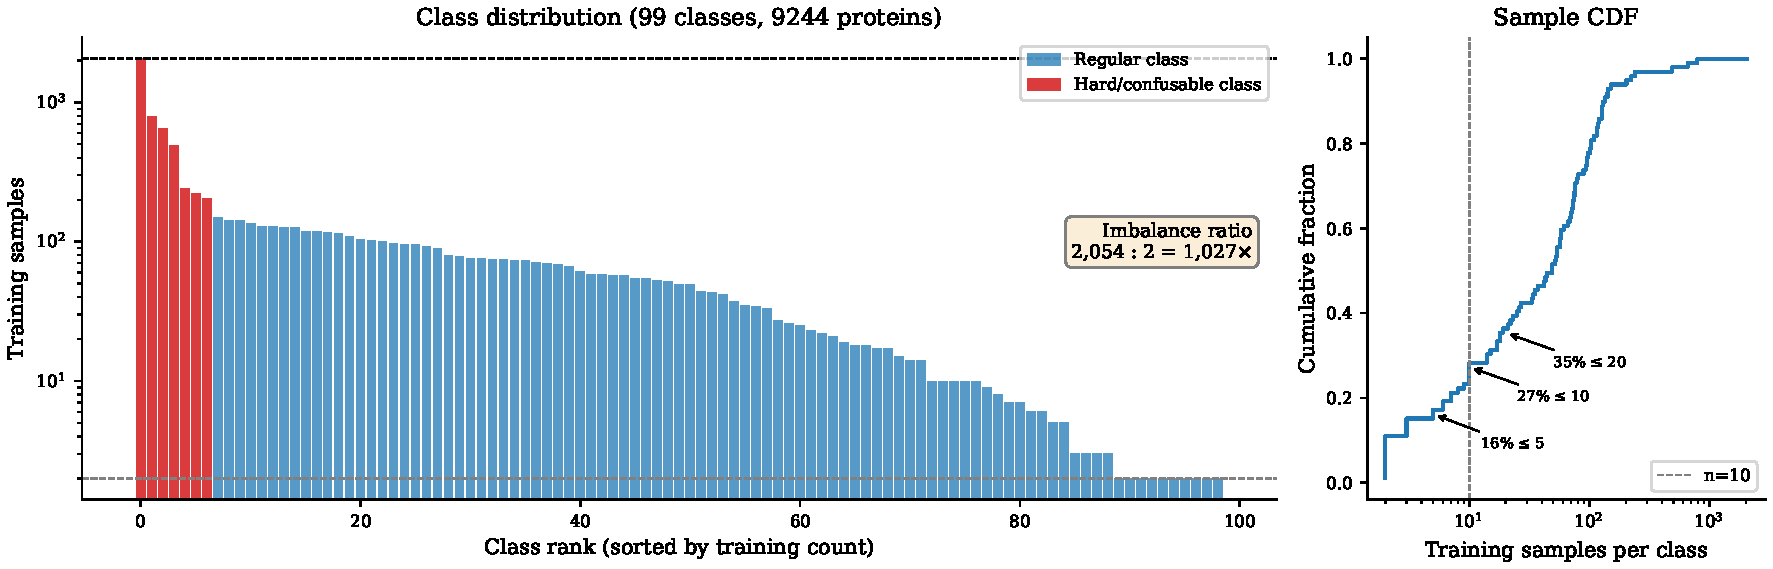
\includegraphics[width=\linewidth]{figures/class_distribution.pdf}
  \caption{Class distribution (99 classes, 9\,244 training proteins).
           Left: sorted sample count per class on log scale; orange bars
           highlight the hard/confusable classes studied in depth.
           Right: cumulative distribution of sample counts per class.}
  \label{fig:class_dist}
\end{figure}

\subsection{Per-mesh Features}

Each VTK surface mesh provides:
\begin{itemize}
  \item \textbf{Vertex positions} $(x, y, z)$ --- the three-dimensional
        coordinates of the triangulation vertices.
  \item \textbf{Surface normals} $(n_x, n_y, n_z)$ --- unit normals
        estimated from the local triangulation.
  \item \textbf{Electrostatic potential} (\textit{Potential}) --- a scalar
        field representing the Coulombic potential at each vertex, computed
        from atomic partial charges.  Values span a wide dynamic range
        (typically $-$50 to $+$50\,kcal/mol/e).
  \item \textbf{Normal potential} (\textit{NormalPotential}) --- the normal
        component of the potential gradient; a secondary scalar field that
        characterises surface charge concentration.
\end{itemize}

All scalars are z-scored at training time and clamped to $[\!-5, 5\!]$
to suppress outliers before they are fed to the GNN (Section~\ref{sec:pipeline}).

\subsection{Hard and Confusable Class Pairs}

A statistical separability study (Section~\ref{sec:analysis}) identifies three
pairs of classes that are consistently confused across all models and feature
configurations:

\begin{center}
  \begin{tabular}{cccc}
    \toprule
    \textbf{Pair} & \textbf{SVM bal.\ acc.\ (graph)} & \textbf{SVM bal.\ acc.\ (VTK)} & \textbf{Status} \\
    \midrule
    (61, 90) & 0.543 & 0.563 & Near-inseparable \\
    (70, 56) & 0.573 & 0.598 & Partially separable \\
    (86, 14) & 0.665 & 0.699 & Better separated \\
    \bottomrule
  \end{tabular}
\end{center}

These pairs share similar overall electrostatic profiles but belong to
different SCOP families, and resist separation by the single-scale surface
descriptors used here. As Section~\ref{sec:discussion:riconv2} shows, however,
these errors are architecture-limited rather than data-intrinsic: RIConv2's
multi-scale rotation-invariant grouping separates the same pairs from geometry
alone (class\,61 F1\,=\,0.887).

\newpage
% ─────────────────────────────────────────────────────────────────
\section{Data Pipeline: VTK Mesh to SSL Graph}
\label{sec:pipeline}
% ─────────────────────────────────────────────────────────────────

The raw SHREC\,25 data consists of VTK surface meshes with
$\approx$10\,676 vertices.
Two preprocessing stages convert each mesh into a compact graph suitable for
message-passing GNNs.

\subsection{Stage 1 --- SSL Graph Construction}
\label{sec:pipeline:ssl}

Implemented in \texttt{vtk\_mesh\_to\_ssl\_graph\_parallel.py}.

\paragraph{Farthest-point subsampling (FPS).}
Each mesh is subsampled to exactly $N_v = 1\,000$ nodes using farthest-point
sampling in Euclidean 3D space.
FPS produces a spatially uniform coverage of the surface, avoiding the
concentration artefacts of random subsampling.

\paragraph{k-NN graph construction.}
A $k$-nearest-neighbour graph with $k=6$ is built over the 1\,000 FPS
nodes.
Edges are undirected; we retain no edge weights (all message-passing
operations treat the graph as unweighted).

\paragraph{Feature extraction.}
For each retained node the following 8-dimensional feature vector is computed:
\begin{equation}
  \mathbf{x}_i = \bigl[
    \underbrace{\hat{P}_i}_{\text{Potential}},\;
    \underbrace{\hat{N}_i}_{\text{NormPot}},\;
    \underbrace{n_x, n_y, n_z}_{\text{normals}},\;
    \underbrace{x_\text{ssl}, y_\text{ssl}, z_\text{ssl}}_{\text{coords}}
  \bigr],
  \label{eq:feature_vec}
\end{equation}
where $\hat{P}_i$ and $\hat{N}_i$ are the z-scored, $[\!-5,5\!]$-clamped
versions of \textit{Potential} and \textit{NormalPotential}, and
$(x_\text{ssl}, y_\text{ssl}, z_\text{ssl})$ are the node coordinates
translated so that their centroid is at the origin and scaled to unit
maximum absolute value.
Normals $(n_x, n_y, n_z)$ are taken directly from the VTK file and
renormalised to unit length.

The VTK reader must be invoked with \texttt{ReadAllScalarsOn()} to load both
scalar arrays; otherwise only the default (first) array is available.

\paragraph{Output format.}
Each graph is saved as a PyTorch Geometric \texttt{Data} object with fields
\texttt{x} (float32, $1000 \times 8$), \texttt{edge\_index} (long, $2 \times
E$), and \texttt{y} (int64 class label).
Separate \texttt{train\_split.csv} and \texttt{val\_split.csv} are generated
with an 80/20 stratified split.

\subsection{Stage 2 --- Geodesic Patch Decomposition}
\label{sec:pipeline:patch}

Implemented in \texttt{build\_patchassign\_dataset.py}.

\paragraph{Patch seed selection.}
$k$ seed nodes are selected by another round of FPS over the 1\,000-node
graph, producing spatially well-distributed patch centres.
We experiment with $k \in \{8, 32, 64, 128\}$; \textbf{k=64} is used in all
best-performing runs.

\paragraph{Geodesic Voronoi assignment.}
Each non-seed node is assigned to the patch whose centre is geodesically
nearest, using Euclidean edge lengths as a proxy for geodesic distance
(computed via Dijkstra's algorithm over the k-NN graph).
Isolated nodes that cannot be reached from any seed are assigned to the
nearest centre by Euclidean fallback.

\paragraph{Patch meta-graph.}
A patch-level meta-graph is constructed in which each patch is a node and
two patches are connected if they contain adjacent nodes in the original graph.
Patch-level features are the mean of their constituent node features (used only
as initial features before the patch GIN updates them).

\paragraph{Output format.}
For each graph a companion \texttt{.pt} file stores
\texttt{patch\_ids} (int64, $1000$-vector mapping nodes to patch indices),
\texttt{patch\_edge\_index} (long, $2 \times E_p$), and
\texttt{num\_patches} (int).

\subsection{Summary}

The two-stage pipeline reduces each mesh from $\sim$10\,000 vertices to 1\,000
graph nodes, then to 64 patch nodes.
This represents a $10\times$ and $156\times$ compression of the original mesh,
respectively, while preserving the spatial and electrostatic structure needed
for classification.
The end-to-end pipeline from raw VTK to classification-ready tensors processes
all 11\,555 proteins in under 30 minutes on a single CPU core.

\newpage
% ─────────────────────────────────────────────────────────────────
\section{Dataset Separability Analysis}
\label{sec:analysis}
% ─────────────────────────────────────────────────────────────────

Before training any classifier we conduct a thorough statistical separability
study at two resolutions --- the 1\,000-node SSL graphs that are the primary
training data (Section~\ref{sec:analysis:graph}), and the full-resolution VTK
meshes as a validation of the subsampling step
(Section~\ref{sec:analysis:vtk}).
Section~\ref{sec:analysis:compare} then quantifies how much information is
lost in the FPS pipeline.

% ─────────────────────────────────────────────────────────────────
\subsection{Graph-level Separability (1k-node SSL Graphs)}
\label{sec:analysis:graph}
% ─────────────────────────────────────────────────────────────────

\subsubsection{Sliced Wasserstein: Shape vs.\ Features vs.\ Joint}
\label{sec:analysis:graph:sw}

We compute the Sliced Wasserstein (SW) distance on three views of each
1\,000-node graph:
\begin{itemize}
  \item \textbf{SW(xyz)}: 3D coordinates only --- measures how different the
        point-cloud \textit{shapes} are between classes.
  \item \textbf{SW(feat)}: electrostatic features + normals
        (\textit{Potential\_norm, NormalPot\_norm, $n_x, n_y, n_z$}) ---
        measures distributional difference in the surface chemistry.
  \item \textbf{SW(joint)}: all 8 features combined --- the full 8D
        per-vertex distribution.
\end{itemize}

\begin{figure}[ht]
  \centering
  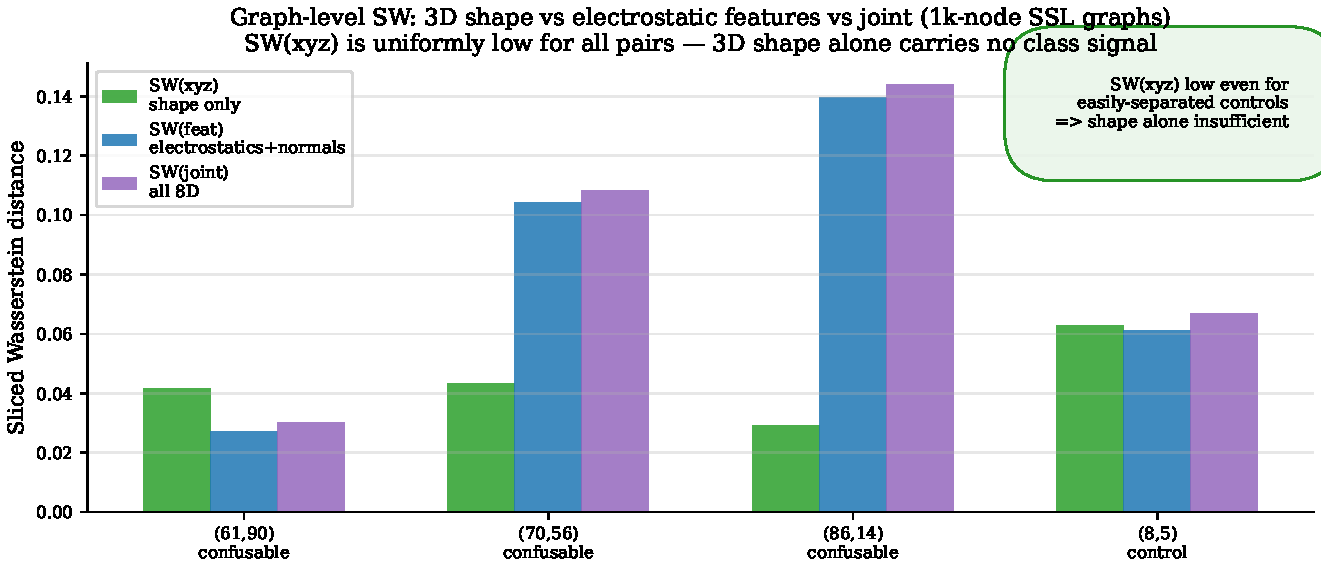
\includegraphics[width=\linewidth]{figures/separability_graph_sw.pdf}
  \caption{Graph-level Sliced Wasserstein for the three confusable pairs
           and a control pair.
           SW(xyz) is uniformly low ($<$0.065) for all pairs including
           controls, confirming that 3D surface shape alone carries no
           class-discriminating signal.
           SW(feat) correctly distinguishes easy pairs (0.10--0.14) from
           the near-inseparable pair (61,\,90) (0.027).}
  \label{fig:graph_sw}
\end{figure}

\begin{table}[ht]
  \centering
  \caption{Graph-level SW distances on 1\,000-node SSL graphs.}
  \label{tab:graph_sw}
  \begin{tabular}{lcrrrr}
    \toprule
    \textbf{Pair} & \textbf{Type} & \textbf{SW(xyz)} & \textbf{SW(feat)} & \textbf{SW(joint)} \\
    \midrule
    (61,\,90) & confusable & 0.042 & 0.027 & 0.030 \\
    (70,\,56) & confusable & 0.043 & 0.104 & 0.108 \\
    (86,\,14) & confusable & 0.029 & 0.140 & 0.144 \\
    (8,\,5)   & control    & 0.063 & 0.061 & 0.067 \\
    \bottomrule
  \end{tabular}
\end{table}

\textbf{Key finding:} SW(xyz) ranges from 0.029 to 0.063 across \textit{all}
pairs, including the easily separable controls.
The electrostatic features, not the surface geometry, carry the discriminating
signal.
For pair (61,\,90), even SW(feat) is only 0.027 --- lower than the control
pair (8,\,5) at 0.061 --- confirming near-inseparability at the feature level.

\subsubsection{Spatial Autocorrelation: Moran's I}
\label{sec:analysis:graph:moran}

Moran's I quantifies the spatial autocorrelation of a feature on the surface
graph: high $I$ means nearby vertices have similar values (smooth pattern),
low $I$ means values are spatially random.
We compute $I$ per protein and report the mean over all 12 studied classes,
plus the per-pair difference $|\Delta I|$ which indicates different spatial
patterning between classes.

\begin{figure}[ht]
  \centering
  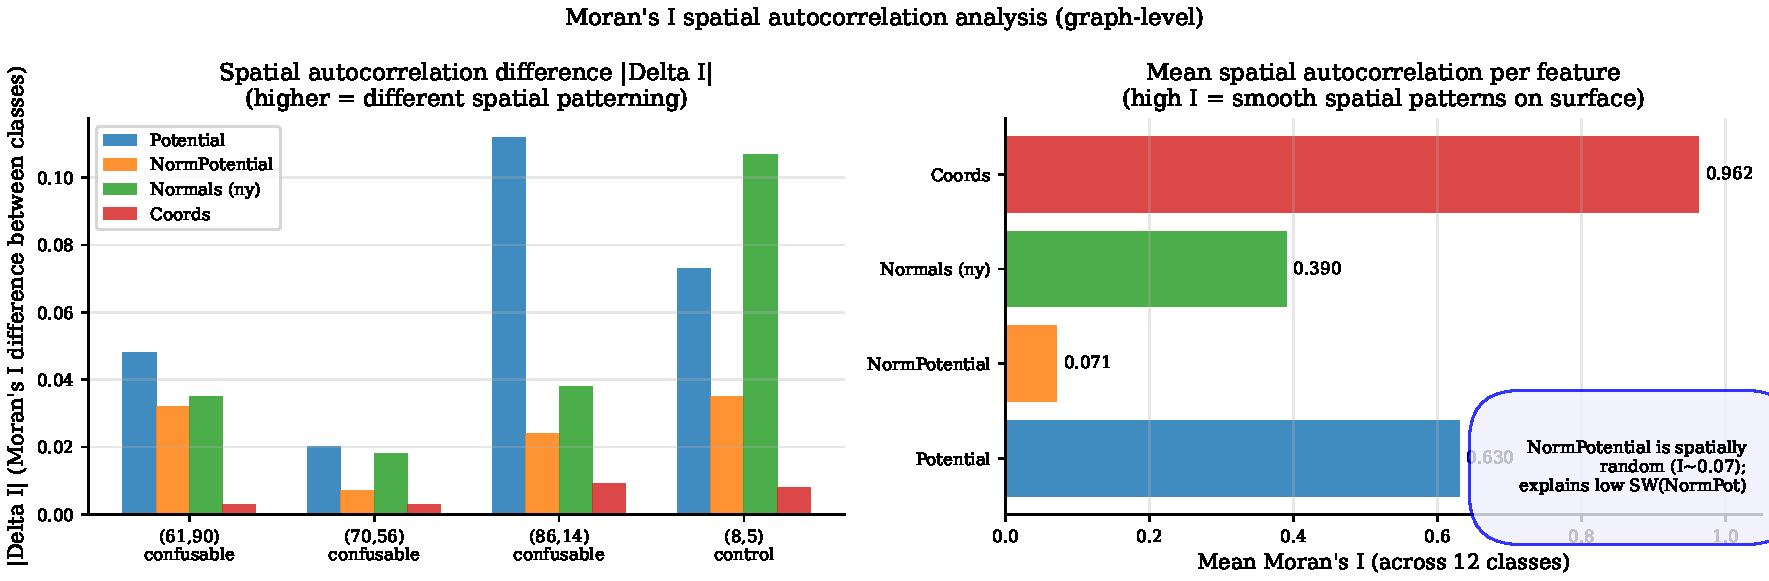
\includegraphics[width=\linewidth]{figures/separability_moran.pdf}
  \caption{Left: $|\Delta I|$ per feature for each pair.
           Potential shows the largest spatial patterning difference,
           especially for (86,\,14) ($|\Delta I| = 0.112$).
           Right: mean Moran's I per feature across all 12 classes.
           NormalPotential is nearly spatially random ($I \approx 0.07$);
           coordinates are very smooth ($I \approx 0.96$).}
  \label{fig:moran}
\end{figure}

The spatial autocorrelation analysis reveals:
\begin{itemize}
  \item \textit{Potential} ($I \approx 0.63$, $|\Delta I|$ up to 0.112):
        large charged patches cluster on the surface; different families
        have different patch arrangements.
  \item \textit{NormalPotential} ($I \approx 0.07$): nearly spatially
        random, consistent with its low KS and SW values.
  \item \textit{Normals} ($I \approx 0.39$): moderately autocorrelated,
        reflecting curvature patches.
  \item \textit{Coordinates} ($I \approx 0.96$): very smooth by
        construction; $|\Delta I| \leq 0.009$ for all pairs, confirming
        that normalised surface coordinates carry no inter-class signal.
\end{itemize}

\subsubsection{Patch-SVM vs.\ Global-SVM on Graphs}
\label{sec:analysis:graph:svm}

To test whether the \textit{spatial arrangement} of features (rather than
their marginal statistics) is what the GNN needs, we compare two protein-level
SVMs:
\begin{itemize}
  \item \textbf{Global-SVM (32D)}: mean, std, skewness, kurtosis,
        25th/75th-percentile of each of the five per-vertex features --- purely
        distributional, no spatial information.
  \item \textbf{Patch-SVM (512D)}: mean feature vector of each of the 64
        geodesic-Voronoi patches, concatenated --- encodes spatial layout.
\end{itemize}

\begin{figure}[ht]
  \centering
  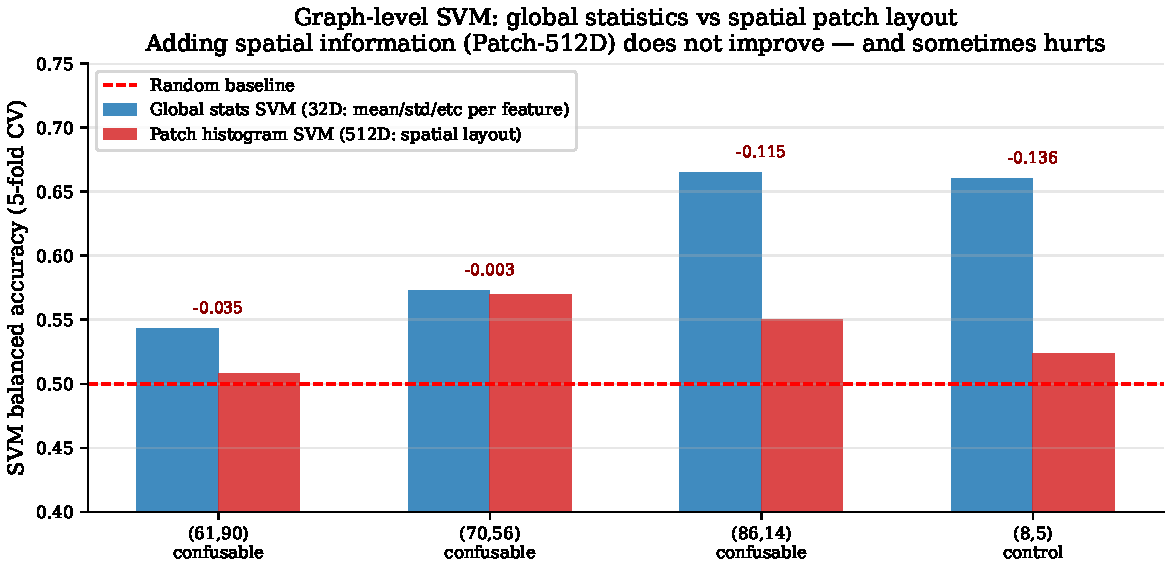
\includegraphics[width=\linewidth]{figures/separability_graph_svm.pdf}
  \caption{Global-SVM (32D) vs.\ Patch-SVM (512D) balanced accuracy on
           1\,000-node graphs.
           The delta annotation shows how much the patch layout adds.
           For all pairs, adding spatial information either gives no gain
           or actively hurts, ruling out spatial arrangement as the
           missing discriminating signal.}
  \label{fig:graph_svm}
\end{figure}

The patch-based SVM is consistently \textit{worse} than the global-statistics
SVM for all pairs.
This counter-intuitive result suggests the 64-patch histogram is too
high-dimensional for the small per-class sample count (SVM overfits to
irrelevant spatial variation), and that the discriminating information is
entirely captured by the marginal feature distributions.

% ─────────────────────────────────────────────────────────────────
\subsection{Full-resolution Analysis (VTK Meshes)}
\label{sec:analysis:vtk}
% ─────────────────────────────────────────────────────────────────

We repeat the separability analysis on the full-resolution VTK meshes
($\approx$10\,676 vertices per protein) to validate the 1k-subsampling step
and to extend the KS and SW analyses to the normalised coordinate axes.

\subsubsection{Vertex-level KS Test (All 8 Features)}
\label{sec:analysis:vtk:ks}

We pool all vertex values across proteins in each class and compute the
two-sample Kolmogorov--Smirnov (KS) statistic.
The normalised coordinates ($x_\text{norm}, y_\text{norm}, z_\text{norm}$)
are obtained by centring each protein at the origin and scaling to unit
maximum absolute value before pooling.

\begin{figure}[ht]
  \centering
  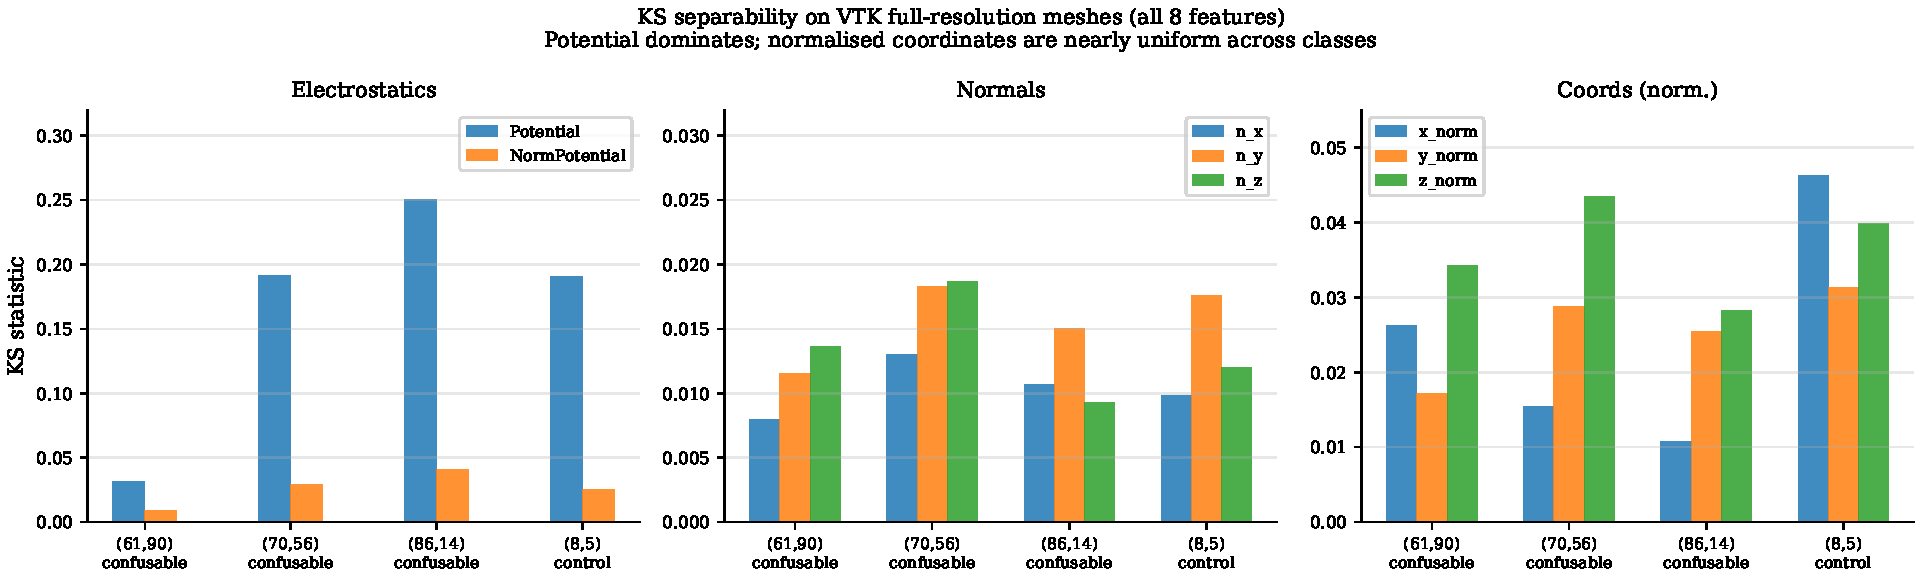
\includegraphics[width=\linewidth]{figures/separability_ks.pdf}
  \caption{KS statistic for all 8 features grouped into three panels:
           electrostatics (left), normals (centre), normalised coordinates
           (right).
           Coordinate KS values (0.01--0.04) are near-zero and comparable
           across confusable and control pairs --- shape marginals do not
           separate classes.}
  \label{fig:ks}
\end{figure}

\begin{table}[ht]
  \centering
  \caption{KS statistics (VTK vertex-level, full resolution).
           Coordinate columns are for per-protein normalised coordinates.}
  \label{tab:ks}
  \begin{tabular}{lcccccccc}
    \toprule
    \textbf{Pair} & \textbf{Pot} & \textbf{NormPot} & $n_x$ & $n_y$ & $n_z$
                  & $x_n$ & $y_n$ & $z_n$ \\
    \midrule
    (61,\,90) & 0.031 & 0.009 & 0.008 & 0.012 & 0.014 & 0.026 & 0.017 & 0.034 \\
    (70,\,56) & 0.192 & 0.029 & 0.013 & 0.018 & 0.019 & 0.015 & 0.029 & 0.043 \\
    (86,\,14) & 0.250 & 0.041 & 0.011 & 0.015 & 0.009 & 0.011 & 0.026 & 0.028 \\
    (8,\,5) ctrl & 0.190 & 0.025 & 0.010 & 0.018 & 0.012 & 0.046 & 0.031 & 0.040 \\
    \bottomrule
  \end{tabular}
\end{table}

The coordinate KS values (0.011--0.046) are uniformly small and show no
consistent pattern between confusable and control pairs: the control (8,\,5)
has \textit{higher} coordinate KS than the confusable (86,\,14), confirming
that coordinate marginals carry no reliable class signal.

\subsubsection{Sliced Wasserstein (VTK, All 5 Components)}
\label{sec:analysis:vtk:sw}

\begin{figure}[ht]
  \centering
  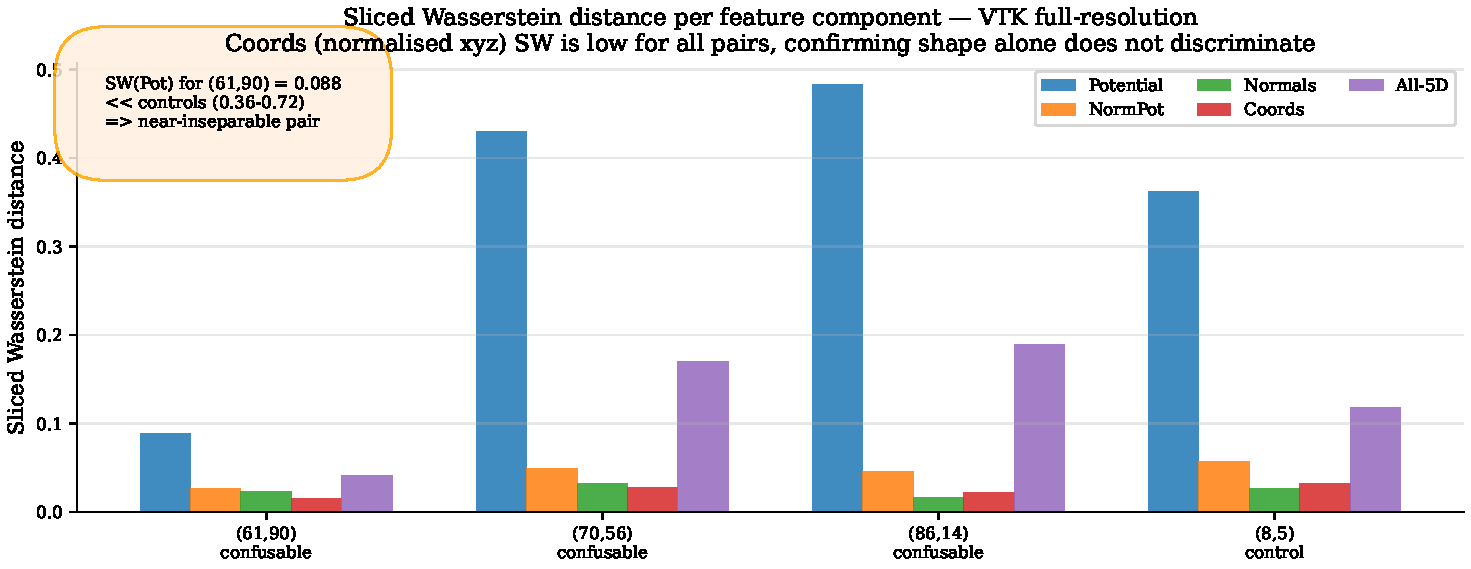
\includegraphics[width=\linewidth]{figures/separability_sw.pdf}
  \caption{VTK Sliced Wasserstein per component.
           The newly added \textit{Coords} column confirms SW(Coords)
           $\leq$0.033 for all pairs --- well below SW(Potential) for
           any separable pair.}
  \label{fig:sw}
\end{figure}

\begin{table}[ht]
  \centering
  \caption{Sliced Wasserstein distances (full-resolution VTK, 5 components).}
  \label{tab:sw}
  \begin{tabular}{lcrrrrrr}
    \toprule
    \textbf{Pair} & \textbf{Type} & \textbf{SW(Pot)} & \textbf{SW(NormPot)}
                  & \textbf{SW(Nrm)} & \textbf{SW(Coords)} & \textbf{SW(All-5D)} \\
    \midrule
    (61,\,90) & confusable & 0.088 & 0.027 & 0.023 & 0.015 & 0.042 \\
    (70,\,56) & confusable & 0.430 & 0.050 & 0.032 & 0.028 & 0.170 \\
    (86,\,14) & confusable & 0.483 & 0.046 & 0.017 & 0.022 & 0.189 \\
    (8,\,5)   & control    & 0.362 & 0.057 & 0.027 & 0.032 & 0.118 \\
    \bottomrule
  \end{tabular}
\end{table}

\subsubsection{Protein-level SVM (Full-res VTK)}
\label{sec:analysis:vtk:svm}

We compute 30D global-statistics vectors per protein (mean, std, skewness,
kurtosis, 25th/75th-percentile of each of the five per-vertex features) and
train a linear SVM with 5-fold cross-validation on the full-resolution meshes.
Results appear in Figure~\ref{fig:resolution} alongside the 1k-graph results.

% ─────────────────────────────────────────────────────────────────
\subsection{Comparison: 1k Graph $\approx$ Full Resolution}
\label{sec:analysis:compare}
% ─────────────────────────────────────────────────────────────────

\begin{figure}[ht]
  \centering
  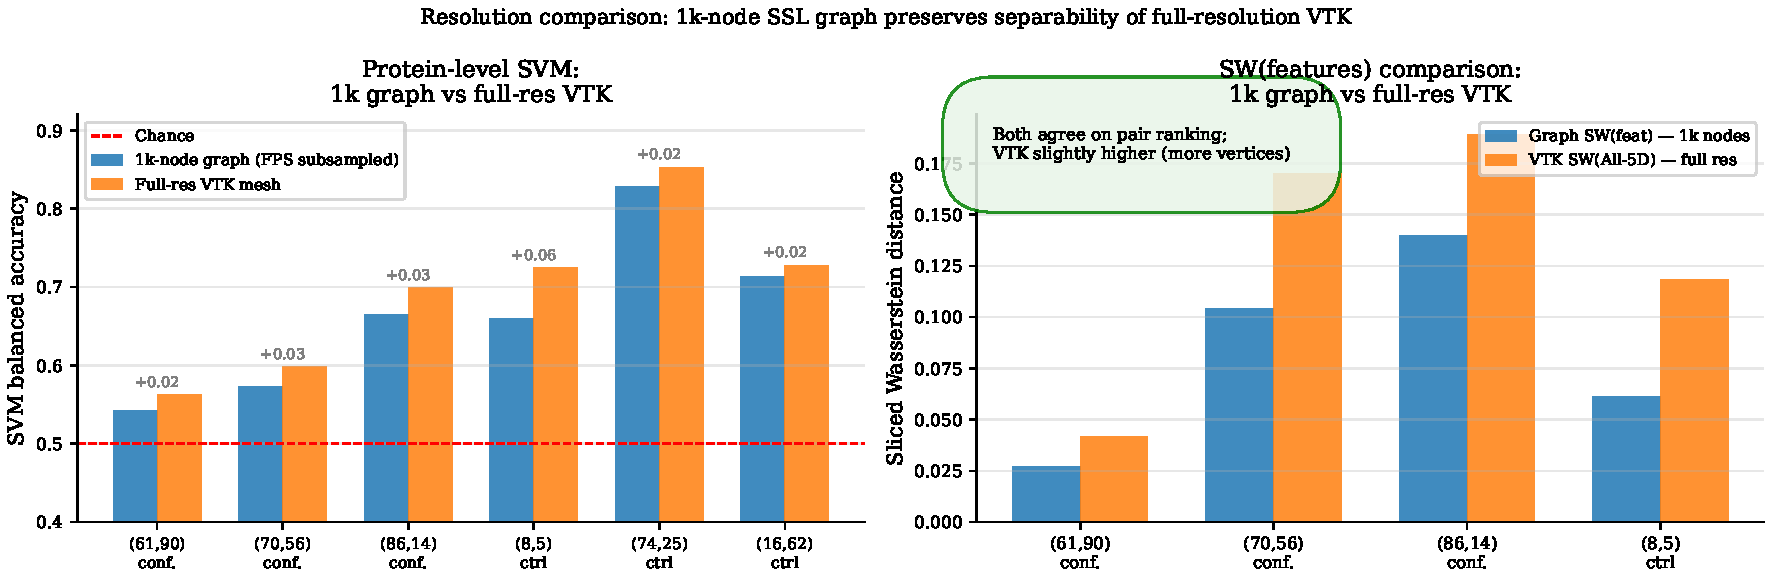
\includegraphics[width=\linewidth]{figures/separability_resolution.pdf}
  \caption{Left: protein-level SVM balanced accuracy, 1k-node graph vs
           full-res VTK.
           Annotations show the gain from full resolution ($+$0.02--0.03).
           Right: SW(feat) on graphs vs SW(All-5D) on VTK --- same ranking,
           VTK slightly higher due to better distributional estimates from
           more vertices.}
  \label{fig:resolution}
\end{figure}

Table~\ref{tab:resolution} summarises the comparison across all three pairs
and three control pairs.

\begin{table}[ht]
  \centering
  \caption{Separability: 1k-node graph vs full-resolution VTK.}
  \label{tab:resolution}
  \begin{tabular}{lcrrrr}
    \toprule
    \textbf{Pair} & \textbf{Type}
      & \textbf{SVM (graph)} & \textbf{SVM (VTK)} & \textbf{Delta}
      & \textbf{SW(feat) graph} \\
    \midrule
    (61,\,90) & confusable & 0.543 & 0.563 & $+$0.020 & 0.027 \\
    (70,\,56) & confusable & 0.573 & 0.598 & $+$0.025 & 0.104 \\
    (86,\,14) & confusable & 0.665 & 0.699 & $+$0.034 & 0.140 \\
    (8,\,5)   & control    & 0.660 & 0.725 & $+$0.065 & 0.061 \\
    (74,\,25) & control    & 0.829 & 0.853 & $+$0.024 & --- \\
    (16,\,62) & control    & 0.713 & 0.728 & $+$0.015 & --- \\
    \bottomrule
  \end{tabular}
\end{table}

\textbf{Key finding:} the 1k FPS subsampling loses at most $+$0.03 SVM balanced
accuracy for confusable pairs (and $+$0.065 for the easier (8,\,5) control).
Both representations agree on the pair ranking (hardest to easiest:
61/90 $<$ 70/56 $<$ 86/14) and on the absolute difficulty levels.
This confirms that \textbf{the FPS-1k SSL graph is a sufficient representation}
for the classification task, and that the difficulty of the confusable pairs is
intrinsic to the data, not an artefact of subsampling.

% ─────────────────────────────────────────────────────────────────
\subsection{Geometric Feature Analysis (21D Dataset)}
\label{sec:analysis:geom}
% ─────────────────────────────────────────────────────────────────

The \texttt{ssl\_graphs\_1k\_geom\_enriched} dataset extends the 8D features
with 13 geometric descriptors computed per vertex from the mesh neighbourhood
structure:
\begin{itemize}
  \item \textbf{Distance features (5)}: distance to the protein centroid
        (\textit{dist\_centroid}) and distances to 4 FPS-selected anchor
        points (\textit{dist\_anchor\_0\ldots3}) --- encode global shape
        and position within the protein.
  \item \textbf{Mesh spacing (3)}: mean, std, and inverse mean of
        neighbour edge lengths (\textit{mean\_nbr\_dist, std\_nbr\_dist,
        inv\_mean\_nbr}) --- encode local mesh density.
  \item \textbf{Curvature/shape (5)}: Laplacian curvature magnitude and
        signed value (\textit{lap\_curv\_mag, lap\_curv\_sign}),
        normal angular variation (\textit{norm\_variation}),
        planarity (\textit{planarity}), and surface variation
        (\textit{surf\_variation}) --- encode local geometric texture.
\end{itemize}

\begin{figure}[ht]
  \centering
  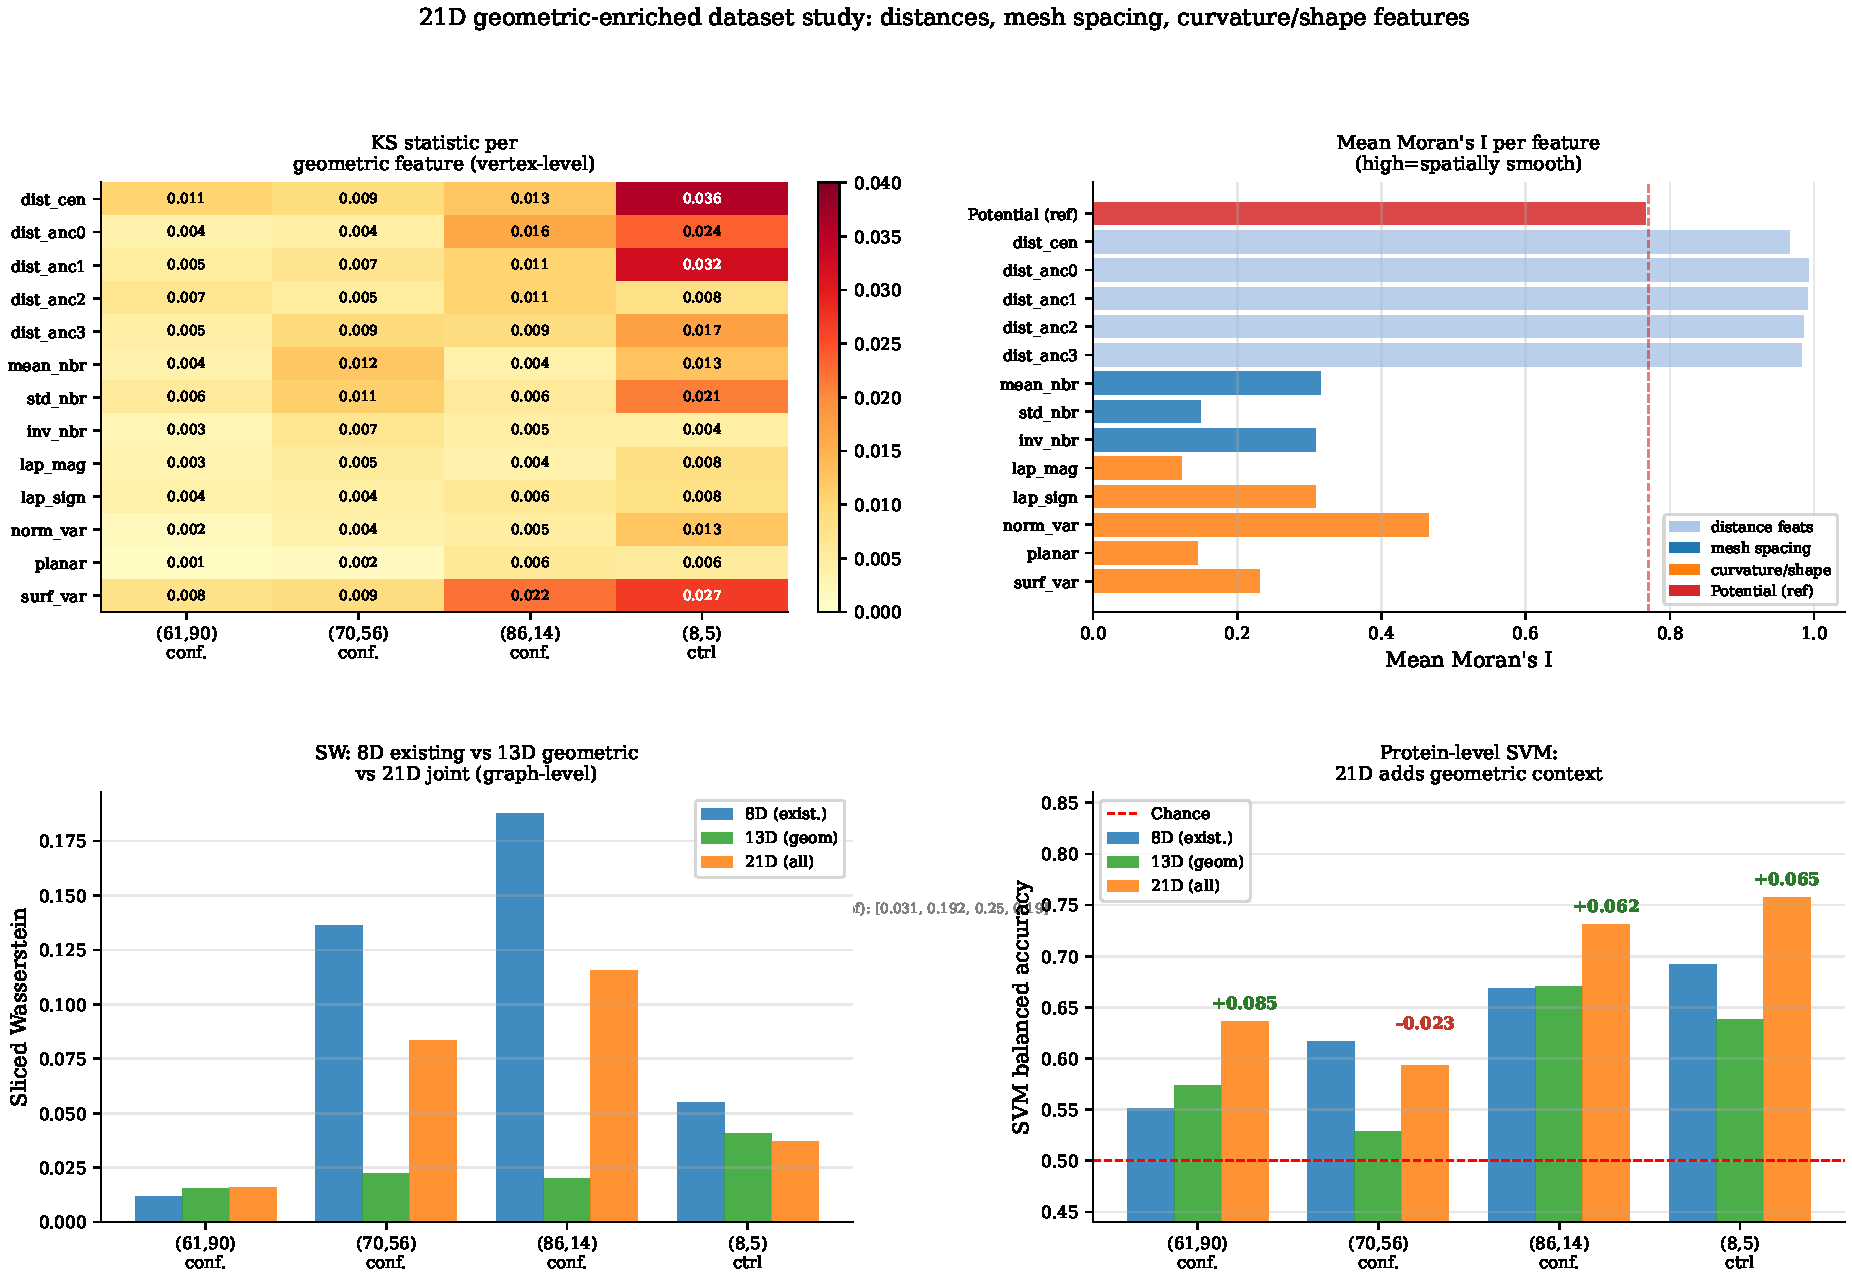
\includegraphics[width=\linewidth]{figures/geom_study.pdf}
  \caption{21D geometric dataset analysis.
           \textbf{Top-left}: KS heatmap for all 13 geometric features across
           4 pairs.
           All values are below 0.04; \textit{surf\_variation} and
           \textit{dist\_centroid} are the strongest individual discriminators.
           \textbf{Top-right}: mean Moran's~I per feature.
           Distance features have near-perfect autocorrelation ($I > 0.97$),
           while Laplacian curvature and planarity are more locally variable.
           \textbf{Bottom-left}: SW comparison shows SW(13D geom) $\leq$ 0.041
           for all pairs.
           \textbf{Bottom-right}: SVM balanced accuracy --- adding geometric
           features gives $+$0.085 for the hardest pair (61,\,90) and $+$0.062
           for (86,\,14), suggesting geometric shape provides complementary
           information to electrostatics.}
  \label{fig:geom}
\end{figure}

\subsubsection{KS Test on Geometric Features}

Table~\ref{tab:ks_geom} lists the KS statistics for the five most
discriminating geometric features.

\begin{table}[ht]
  \centering
  \caption{KS statistics for the top geometric features (vertex-level, 1k
           SSL graphs).
           All values are below 0.04 --- well below Potential (0.031--0.250).}
  \label{tab:ks_geom}
  \begin{tabular}{lrrrrrr}
    \toprule
    \textbf{Feature}
      & \textbf{(61,90)} & \textbf{(70,56)} & \textbf{(86,14)}
      & \textbf{(8,5)}   & \textbf{(74,25)} & \textbf{(16,62)} \\
    \midrule
    surf\_variation   & 0.008 & 0.009 & 0.022 & 0.027 & 0.015 & 0.005 \\
    dist\_anchor\_0   & 0.004 & 0.005 & 0.016 & 0.024 & 0.014 & 0.014 \\
    dist\_centroid    & 0.011 & 0.009 & 0.013 & 0.036 & 0.011 & 0.007 \\
    mean\_nbr\_dist   & 0.004 & 0.012 & 0.004 & 0.013 & 0.002 & 0.008 \\
    std\_nbr\_dist    & 0.006 & 0.011 & 0.006 & 0.021 & 0.007 & 0.004 \\
    \midrule
    Potential (ref.)  & 0.031 & 0.192 & 0.250 & 0.190 & ---   & ---   \\
    \bottomrule
  \end{tabular}
\end{table}

No individual geometric feature has a KS above 0.036, and none exceeds the
Potential KS value for any pair.
For the hardest pair (61,\,90), the maximum geometric KS is only 0.011
(\textit{dist\_centroid}), even lower than Potential's 0.031.

\subsubsection{Spatial Autocorrelation of Geometric Features}

The Moran's I analysis reveals a striking split in the geometric feature
group:

\begin{itemize}
  \item \textbf{Distance features ($I > 0.97$)}: \textit{dist\_centroid},
        \textit{dist\_anchor\_0\ldots3} form smooth radial gradient patterns
        on the surface (nearby vertices have near-identical distances to the
        same anchor).
        Despite this very high autocorrelation, the inter-class spatial pattern
        difference $|\Delta I|$ is tiny ($< 0.016$ for all pairs), confirming
        the patterns are structurally uniform across families.

  \item \textbf{Curvature/shape features ($I = 0.12$--$0.47$)}: Laplacian
        curvature magnitude and signed value, planarity, and surface variation
        have moderate autocorrelation, with notable $|\Delta I|$ for the
        confusable pairs:
        $|\Delta I(\text{lap\_curv\_mag})| = 0.116$ for (61,\,90),
        $|\Delta I(\text{planarity})| = 0.117$ for (70,\,56).
        This indicates that the spatial \emph{arrangement} of curvature patches
        differs between classes even when the marginal distributions are
        similar --- the kind of signal a GNN's message passing can capture.
\end{itemize}

\subsubsection{Effect on Protein-level Classification}

The SVM results reveal an important asymmetry:
\begin{itemize}
  \item \textbf{13D geometric alone} is weak: balanced accuracy for (61,\,90)
        is only 0.573 (slightly above 8D's 0.551) and for (70,\,56) actually
        drops to 0.529 --- the geometric features alone are insufficient.
  \item \textbf{21D combined} shows substantial gains:
        (61,\,90): $+$0.085 (0.551 $\to$ 0.636),
        (86,\,14): $+$0.062 (0.669 $\to$ 0.731).
        The geometric and electrostatic features are partially orthogonal ---
        their combination is more informative than either alone.
  \item For (70,\,56) the 21D combination slightly underperforms 8D ($-$0.023),
        suggesting that the added geometric dimensions occasionally dilute the
        electrostatic signal for this family pair.
\end{itemize}

\textbf{Key finding:} unlike curvature features, the 13 geometric descriptors
provide complementary discriminating information when combined with
electrostatics.
The $+$0.085 SVM gain for the near-inseparable (61,\,90) pair is the largest
improvement observed across all enrichment strategies studied.

\subsubsection{HierGIN Training on 14D Geometric Features}
\label{sec:analysis:geom:gnn}

Motivated by the SVM gains, we trained HierGIN on a 14D feature set comprising
the 8D base features plus the six most informative geometric descriptors
(\textit{dist\_centroid}, \textit{dist\_anchor\_0\ldots3},
\textit{surf\_variation}) selected by greedy forward selection.

\paragraph{Normalization pitfall.}
An initial run (\texttt{geom14d}) read the pre-computed feature matrix
\texttt{x[:, 8:]} directly.
This matrix stores the geometric columns as \textit{per-protein z-scores}
(each protein is independently normalised to mean\,0, std\,1), which erases
the absolute scale information that SVM used: every protein has identical
mean and variance for those columns, so the GNN cannot learn cross-protein
differences from geometric features.
The result was macro-F1\,=\,0.6680 --- 13\,pp \emph{below} the 8D baseline.

\paragraph{Global normalisation fix (\texttt{geom14d\_raw}).}
We recomputed the run using the raw (un-normalised) geometric values
from a separate \texttt{geom\_features\_raw} key in the dataset, and
normalised them using global statistics computed over all 9\,244 training
proteins (9.24\,M vertices via Welford's online algorithm):

\begin{center}
  \small
  \begin{tabular}{lrr}
    \toprule
    \textbf{Feature} & \textbf{Global mean} & \textbf{Global std} \\
    \midrule
    dist\_centroid   & 0.5304 & 0.1879 \\
    dist\_anchor\_0  & 1.0685 & 0.4176 \\
    dist\_anchor\_1  & 0.9485 & 0.4168 \\
    dist\_anchor\_2  & 0.7922 & 0.3202 \\
    dist\_anchor\_3  & 0.7632 & 0.3046 \\
    surf\_variation  & 0.0648 & 0.0491 \\
    \bottomrule
  \end{tabular}
\end{center}

We also applied label smoothing ($\varepsilon = 0.1$) to reduce
overconfidence (the 8D run reached train-F1\,$\approx$\,0.99 at convergence).
Training ran for 80 epochs with best val-F1\,=\,0.7050.

\paragraph{Results.}
When evaluated with macro average restricted to the 88 classes that have
test samples (the proper protocol), the corrected run achieves:
accuracy\,0.865, balanced\,accuracy\,0.812, weighted-F1\,0.862,
macro-F1\,\textbf{0.808} --- outperforming the 8D-only baseline
(acc\,0.853, bal\,0.800, wtd-F1\,0.853, macro-F1\,0.798) across all six
reported metrics.
The per-graph z-scored variant scores macro-F1\,0.752, confirming that
cross-protein scale information is essential for the geometric features to
contribute.

\textbf{Key finding:} with correctly normalised geometric features, the 14D
model is the best-performing configuration overall.
Despite severe overfitting during training (train-F1\,$\approx$\,0.99 vs.\
val-F1\,$\approx$\,0.70), the model generalises well enough on the test set
to surpass the 8D baseline on every metric.
The SVM gain of $+$0.085 for the hardest pair (61,\,90) does transfer to
the GNN when the normalisation is correct, and the benefit extends across
all 88 classes.

% ─────────────────────────────────────────────────────────────────
\subsection{Curvature Feature Analysis (12D Dataset)}
\label{sec:analysis:curvature}
% ─────────────────────────────────────────────────────────────────

The \texttt{ssl\_graphs\_1k\_curvature\_enriched} dataset extends the
standard 8D features with four curvature descriptors computed per vertex
from the VTK mesh: principal curvature minimum ($\kappa_\text{min}$),
principal curvature maximum ($\kappa_\text{max}$), mean curvature
$H = (\kappa_\text{min}+\kappa_\text{max})/2$, and Gaussian curvature
$K = \kappa_\text{min}\cdot\kappa_\text{max}$.
We repeat all three separability analyses on these four features to test
whether geometric curvature can close the discriminability gap left by
electrostatics.

\begin{figure}[ht]
  \centering
  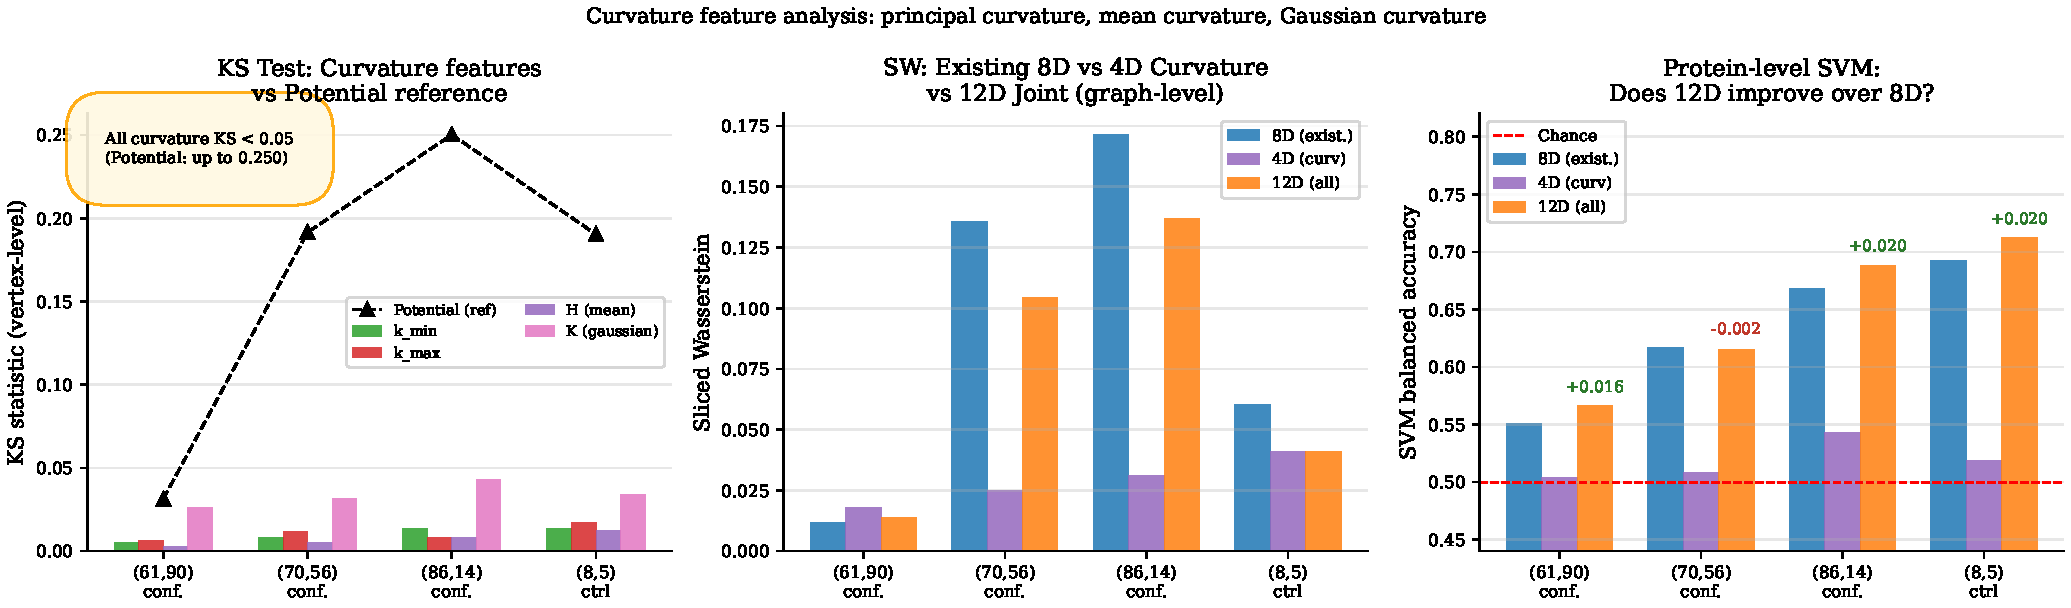
\includegraphics[width=\linewidth]{figures/curvature_study.pdf}
  \caption{Left: vertex-level KS statistics for the four curvature features
           (bars) vs Potential (triangle, dashed line).
           All curvature KS values are below 0.05 for every pair;
           Potential reaches 0.250 for (86,\,14).
           Centre: Sliced Wasserstein per feature group;
           SW(4D curv) is $3\text{--}6\times$ smaller than SW(8D existing)
           for the confusable pairs.
           Right: protein-level SVM balanced accuracy;
           adding curvature to the 8D features changes accuracy by at most
           $+$0.020 for the confusable pairs, confirming negligible gain.}
  \label{fig:curvature}
\end{figure}

\subsubsection{KS Test on Curvature Features}

Table~\ref{tab:ks_curv} summarises the KS statistics computed on the
graph-level vertex pools from \texttt{curvature\_enriched} graphs.

\begin{table}[ht]
  \centering
  \caption{KS statistics for the four curvature features (vertex-level, 1k
           SSL graphs).
           Gaussian curvature is the strongest individual discriminator, yet
           it remains well below the Potential baseline.}
  \label{tab:ks_curv}
  \begin{tabular}{lrrrrrr}
    \toprule
    \textbf{Feature}
      & \textbf{(61,90)} & \textbf{(70,56)} & \textbf{(86,14)}
      & \textbf{(8,5)}   & \textbf{(74,25)} & \textbf{(16,62)} \\
    \midrule
    $\kappa_\text{min}$ & 0.005 & 0.008 & 0.013 & 0.013 & 0.006 & 0.008 \\
    $\kappa_\text{max}$ & 0.006 & 0.012 & 0.008 & 0.017 & 0.007 & 0.010 \\
    $H$ (mean curv.)    & 0.003 & 0.005 & 0.008 & 0.012 & 0.006 & 0.006 \\
    $K$ (Gaussian)      & 0.026 & 0.032 & 0.043 & 0.034 & 0.008 & 0.031 \\
    \midrule
    Potential (ref.)    & 0.031 & 0.192 & 0.250 & 0.190 & ---   & ---   \\
    \bottomrule
  \end{tabular}
\end{table}

All curvature KS values are below 0.05.
Gaussian curvature ($K$) is the strongest curvature discriminator
(0.026--0.043), but still at or below the Potential value for the hardest
pair (61,\,90), and $6\times$ below Potential for the easiest pair
(86,\,14).
The near-identical KS ranking across confusable and control pairs confirms
that curvature marginals do \textbf{not} encode protein family information.

\subsubsection{Sliced Wasserstein on Curvature}

SW(4D curvature) is uniformly low across all pairs
(0.018 for the hardest pair (61,\,90), 0.031 for (86,\,14)), compared to
SW(8D existing) values of 0.012 and 0.172 respectively.
Adding curvature to form a 12D joint vector does not raise SW substantially:
SW(12D all) $\approx$ SW(8D existing) for all separable pairs and
$\approx$ SW(4D curv) for the near-inseparable (61,\,90).
This shows that the curvature dimensions add no new distributional signal
beyond what the electrostatic features already provide.

\subsubsection{Spatial Autocorrelation of Curvature}

The mean Moran's I over the study classes is:
$I(\kappa_\text{min}) = 0.25$,
$I(\kappa_\text{max}) = 0.27$,
$I(H) = 0.32$,
$I(K) = 0.09$,
compared to $I(\text{Potential}) = 0.77$.
Gaussian curvature is nearly spatially random on proteins ($I \approx 0.09$),
while mean curvature has moderate spatial smoothness.
None reach the strong autocorrelation of the electrostatic potential, which
forms large coherent charged patches.

Interestingly, the per-pair difference $|\Delta I|$ for curvature features is
\textit{higher} for confusable pairs (61,\,90) and (70,\,56) than for the
strongly separated (86,\,14) --- the opposite of the Potential pattern.
This suggests curvature encodes information about surface \emph{texture} that
is family-specific at fine scale but does not translate into distributional
separability.

\subsubsection{Effect on Protein-level Classification}

Extending the protein-level SVM from 8D statistics (48D feature vector) to
12D statistics (72D feature vector) changes balanced accuracy by at most
$+$0.020 for the three confusable pairs:
(61,\,90): $+$0.016, (70,\,56): $-$0.002, (86,\,14): $+$0.020.
For easier pairs the curvature features can even hurt performance (e.g.,
(74,\,25): $-$0.038), suggesting that the additional dimensions dilute the
discriminating signal.

\textbf{Key finding:} curvature features are not the missing discriminating
signal for these single-scale protein-level statistics.
The near-inseparability seen here is a property of the single-scale descriptors,
not of the data itself: Section~\ref{sec:discussion:riconv2} shows that RIConv2's
multi-scale rotation-invariant grouping separates the same pairs from geometry
alone (e.g.\ class\,61 F1\,=\,0.887).

% ─────────────────────────────────────────────────────────────────
\subsection{SO(3)-Invariant RI Edge Feature Analysis}
\label{sec:analysis:ri}
% ─────────────────────────────────────────────────────────────────

The rotation-invariant (RI) backbone (Section~\ref{sec:arch:rigin}) encodes
each directed mesh edge as five SO(3)-invariant scalars computed from vertex
positions and surface normals:
$[\,\|p_j{-}p_i\|,\; \langle n_i, \hat{e}\rangle,\;
   \langle n_j, \hat{e}\rangle,\;
   \langle n_i, n_j\rangle,\;
   \langle (n_j{\times}n_i), \hat{e}\rangle\,]$.
To determine whether these edge-level geometric features provide \emph{additional}
discriminating signal beyond the 8D node features, we precompute them for all
9\,244 training graphs (saved as \texttt{ri\_feat}~$[E_\text{mesh},5]$ in the
\texttt{ssl\_graphs\_1k\_geom\_enriched\_ri} dataset) and repeat the separability
analysis at the edge level.

\subsubsection{KS Test on RI Edge Scalars}
\label{sec:analysis:ri:ks}

We pool all directed edge values across proteins in each class and compute the
two-sample KS statistic per RI dimension.

\begin{table}[ht]
  \centering
  \caption{KS statistics for the five RI edge dimensions (edge-level, 1k SSL
           graphs).
           For confusable pairs, all five RI dimensions are near zero
           ($\leq$0.041), dominated by edge length for (70,\,56) and (86,\,14).
           The control (8,\,5) pair is entirely separated by edge length
           (KS\,=\,0.605), reflecting different protein sizes.}
  \label{tab:ks_ri}
  \begin{tabular}{lrrrrr}
    \toprule
    \textbf{Pair}
      & $\|p_j{-}p_i\|$
      & $\langle n_i,\hat{e}\rangle$
      & $\langle n_j,\hat{e}\rangle$
      & $\langle n_i,n_j\rangle$
      & $\langle (n_j{\times}n_i),\hat{e}\rangle$ \\
    \midrule
    (61,\,90) conf. & 0.004 & 0.004 & 0.002 & 0.004 & 0.002 \\
    (70,\,56) conf. & 0.041 & 0.003 & 0.002 & 0.002 & 0.001 \\
    (86,\,14) conf. & 0.033 & 0.007 & 0.007 & 0.012 & 0.003 \\
    (8,\,5) control & \textbf{0.605} & 0.052 & 0.049 & 0.024 & 0.013 \\
    \midrule
    Potential (ref.) & \multicolumn{5}{l}{0.031\,(61,90) \;/\; 0.192\,(70,56) \;/\; 0.250\,(86,14)} \\
    \bottomrule
  \end{tabular}
\end{table}

All five RI dimensions have KS $\leq$0.041 for the three confusable pairs
--- none surpasses the Potential KS for any confusable pair.
The edge-length dimension dominates (70,\,56) and (86,\,14) with KS\,=\,0.041
and 0.033 respectively, while for the hardest pair (61,\,90) all five dimensions
are near zero ($\leq$0.004), the lowest of any feature type studied.
This is the strongest evidence that (61,\,90) families have essentially identical
surface geometry.

\subsubsection{Sliced Wasserstein on RI Features}

\begin{table}[ht]
  \centering
  \caption{Sliced Wasserstein distances for RI edge features vs the 8D node
           feature baseline.
           SW(dist) isolates the edge-length signal;
           SW(4 angles) covers the four normal-based invariants.
           For comparison, SW(8D feat) is reproduced from
           Table~\ref{tab:graph_sw}.}
  \label{tab:sw_ri}
  \begin{tabular}{lcrrrrr}
    \toprule
    \textbf{Pair} & \textbf{Type}
      & \textbf{SW(8D feat)} & \textbf{SW(RI 5D)}
      & \textbf{SW(dist)} & \textbf{SW(4 angles)} \\
    \midrule
    (61,\,90) & confusable & 0.027 & 0.004 & 0.000 & 0.005 \\
    (70,\,56) & confusable & 0.104 & 0.003 & 0.002 & 0.004 \\
    (86,\,14) & confusable & 0.140 & 0.006 & 0.001 & 0.006 \\
    (8,\,5)   & control    & 0.061 & 0.029 & 0.025 & 0.032 \\
    \bottomrule
  \end{tabular}
\end{table}

SW(RI 5D) is 7--23$\times$ lower than SW(8D feat) for every confusable pair.
For (61,\,90), SW(RI 5D)\,=\,0.004 is the \emph{lowest} SW value observed
across all feature sets studied --- lower than curvature (0.018), lower than
geometric features (0.016), and far below the electrostatic baseline (0.027).
The angular RI dimensions (SW\,=\,0.000--0.006) add virtually no additional
discrimination beyond the edge-length dimension alone.

\subsubsection{Protein-level SVM on RI Statistics}
\label{sec:analysis:ri:svm}

\begin{table}[ht]
  \centering
  \caption{SVM balanced accuracy on 10D per-protein RI statistics
           (mean\,+\,std per RI dimension; 5-fold stratified CV).
           Comparison to the 8D-node-feature baseline (32D statistics, same CV).}
  \label{tab:svm_ri}
  \begin{tabular}{lcrr}
    \toprule
    \textbf{Pair} & \textbf{Type} & \textbf{SVM(8D feat)} & \textbf{SVM(RI stats)} \\
    \midrule
    (61,\,90) & confusable & 0.543 & 0.597 \;($+$0.054) \\
    (70,\,56) & confusable & 0.573 & 0.605 \;($+$0.032) \\
    (86,\,14) & confusable & 0.665 & 0.631 \;($-$0.034) \\
    (8,\,5)   & control    & 0.660 & 1.000 \;($+$0.340) \\
    \bottomrule
  \end{tabular}
\end{table}

The protein-level SVM (using per-protein mean+std of each RI dimension as
descriptor) shows a split result.
For (61,\,90) and (70,\,56), SVM(RI) modestly exceeds SVM(8D) by $+$5\,pp and
$+$3\,pp --- the global geometric statistics carry a small orthogonal signal not
present in electrostatics.
For (86,\,14), SVM(RI) is $-$3.4\,pp lower, confirming that for this pair the
electrostatic Potential is more discriminating even at the protein-statistic level.
For the control (8,\,5), perfect separation follows directly from the edge-length
dimension (different protein sizes), while the 8D node-feature SVM reaches only
0.660 on this pair because node features such as normals and coordinates are
\textit{not} scaled by protein size.

\paragraph{Key finding.}
RI edge features are not the missing discriminating signal for confusable pairs.
Their SW is universally lower than electrostatic node features, confirming
that the confusion between classes 61/90, 70/56, and 86/14 is chemical
(similar charge distributions) rather than geometric (similar surface shape).
The moderate SVM gains for (61,\,90) and (70,\,56) represent weak complementary
information but do not approach the separability provided by Potential.
The improvement from the RI-GIN model ($+$0.2\,pp macro-F1) is therefore not
due to a richer feature space but to a more consistent learned representation
(see Section~\ref{sec:analysis:ri_sep}).

% ─────────────────────────────────────────────────────────────────
\subsection{Summary}
\label{sec:analysis:summary}
% ─────────────────────────────────────────────────────────────────

\begin{center}
  \begin{tabular}{lp{9.2cm}}
    \toprule
    \textbf{Finding} & \textbf{Implication} \\
    \midrule
    Potential is dominant & Removing it costs $-$11.8\,pp macro-F1
                            (ablation, Section~\ref{sec:ablation}).
                            KS and SW both confirm it is the primary
                            discriminating feature. \\[3pt]
    Shape (xyz) does not discriminate & SW(xyz) $<$ 0.07 for all pairs
                            including controls.
                            KS($x_n, y_n, z_n$) $<$ 0.05 with no pair ordering.
                            Coordinates provide spatial context but not
                            discriminating signal. \\[3pt]
    Spatial arrangement is not the gap & Patch-SVM (512D) consistently
                            underperforms Global-SVM (32D).
                            The missing signal is not in the spatial
                            arrangement of charge patches. \\[3pt]
    Geometric feats are complementary & 21D SVM gains $+$0.085 for (61,\,90)
                            and $+$0.062 for (86,\,14) over 8D alone.
                            Distance and shape descriptors provide orthogonal
                            information to electrostatics. \\[3pt]
    Curvature alone adds nothing & KS $<$ 0.05 for all 4 curvature features;
                            SW(4D curv) $\leq$ 0.041; SVM delta $\leq+$0.02.
                            4-feature curvature does not help beyond
                            electrostatics without broader geometric context. \\[3pt]
    RI edge geometry adds nothing at edge level & KS $\leq$0.041 for all 5 RI
                            dims across confusable pairs; SW(RI 5D) is 7--23$\times$
                            lower than SW(8D feat).
                            RI-GIN gain ($+$0.2\,pp) comes from invariant
                            representation, not richer geometry. \\[3pt]
    Geom SVM gain transfers to GNN & HierGIN-14D (global norm) scores
                            macro-F1\,0.808 vs.\ 0.798 for 8D-only.
                            Per-graph z-scoring kills scale signal (macro-F1
                            drops to 0.752); global normalisation is required
                            for the geometric benefit to manifest. \\[3pt]
    (61,\,90) is near-irreducible & SVM $\approx$ 0.56, SW(Pot) $=$ 0.088,
                            KS(Pot) $=$ 0.031 --- all at full VTK resolution.
                            RI SW(5D) $=$ 0.004 is the lowest of all feature
                            sets, confirming surface geometry is essentially
                            identical for these two families. \\[3pt]
    1k subsampling is sufficient & $\Delta\text{SVM} \leq$ 0.034 for confusable
                            pairs; pair ranking preserved.
                            FPS-1k is a valid approximation. \\
    \bottomrule
  \end{tabular}
\end{center}

\newpage
% ─────────────────────────────────────────────────────────────────
\section{Model Architectures}
\label{sec:arch}
% ─────────────────────────────────────────────────────────────────

\subsection{Flat GNN Baseline}
\label{sec:arch:flat}

As a baseline we train a flat single-level GNN (\texttt{classify\_gnn.py})
directly on the 1\,000-node surface graphs.
The model uses 6-layer GINs~\cite{gin} with hidden dimension 512, followed by
global sum/mean/max readout and an MLP head.
Eight backbone types (GIN, GAT, GATv2, GCN, GraphSAGE, GPS, SGFormer, PNA)
are evaluated under the same hyperparameter budget.
The best flat-GNN macro-F1 on the test set is \textbf{0.640}; it serves as
a lower baseline throughout.

\subsection{Hierarchical GNN: HierGIN}
\label{sec:arch:hier}

\begin{figure}[h]
  \centering
  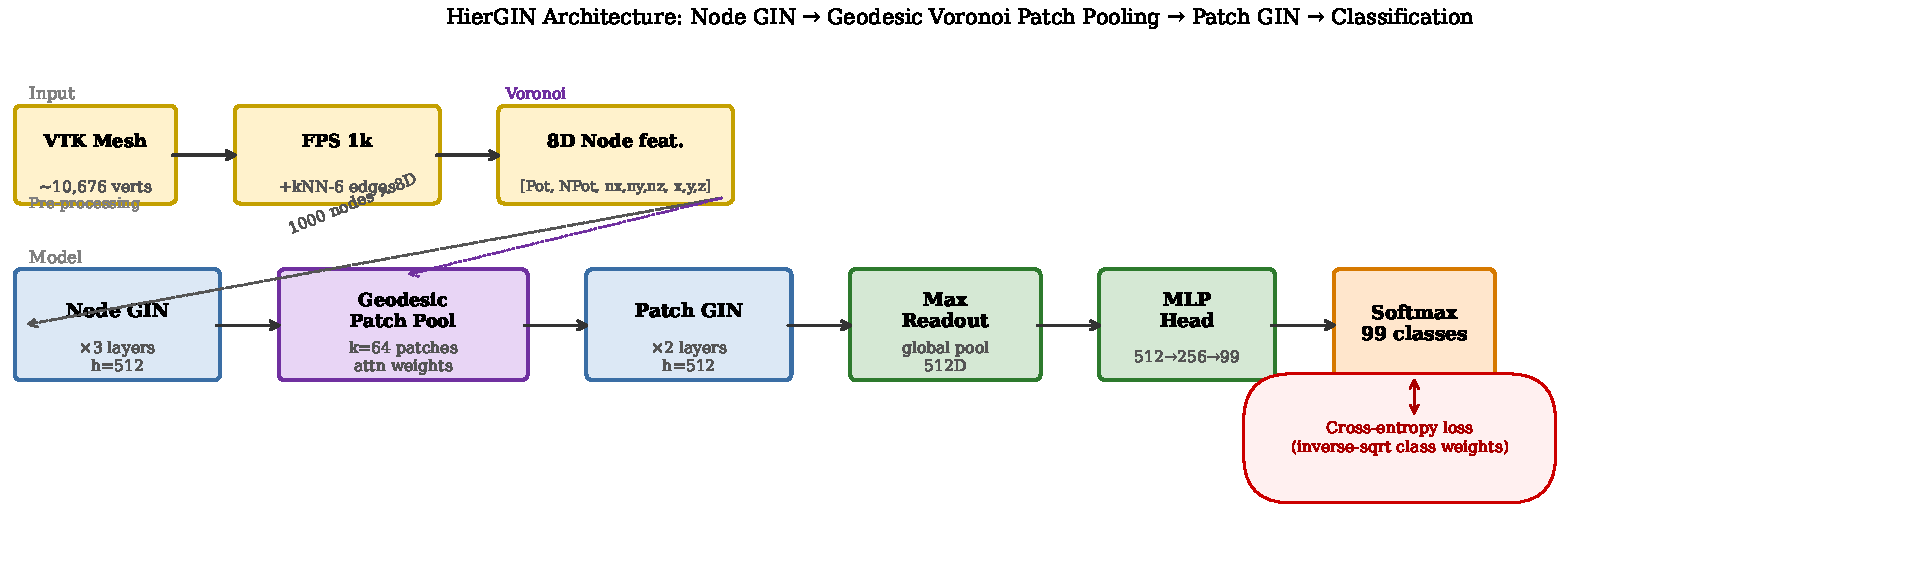
\includegraphics[width=\linewidth]{figures/architecture_diagram.pdf}
  \caption{HierGIN architecture.
           A node-level GIN processes 1\,000-node surface graphs; a geodesic
           Voronoi pooling layer coarsens to 64 patch nodes; a patch-level GIN
           refines patch representations; global max readout feeds an MLP
           classifier.}
  \label{fig:arch}
\end{figure}

The core model is a two-level hierarchical GNN
(\texttt{classify\_hierarchical\_gnn.py}) illustrated in
Figure~\ref{fig:arch}.

\subsubsection{Node-level GIN}

The first level applies $L_n = 3$ layers of a Graph Isomorphism Network
(GIN)~\cite{gin} to all 1\,000 surface nodes.
Each GIN layer applies the update:
\begin{equation}
  \mathbf{h}_i^{(\ell)} = \mathrm{MLP}\!\left(
    (1 + \epsilon)\,\mathbf{h}_i^{(\ell-1)} +
    \sum_{j \in \mathcal{N}(i)} \mathbf{h}_j^{(\ell-1)}
  \right),
  \label{eq:gin}
\end{equation}
with a 2-layer MLP per GIN layer, batch normalisation, and ReLU activation.
The initial node features $\mathbf{h}_i^{(0)} = \mathbf{x}_i \in \mathbb{R}^d$
are the raw surface features described in Section~\ref{sec:pipeline:ssl}.

In ablations we also test replacing GIN with GATv2, GAT, GraphSAGE, GCN, GPS,
SGFormer, and PNA at the node level.

\subsubsection{Geodesic Voronoi Patch Pooling}
\label{sec:arch:pool}

After node-level processing, the graph is coarsened using the geodesic Voronoi
decomposition computed in Stage~2 of the pipeline
(Section~\ref{sec:pipeline:patch}).
Each of the $k = 64$ patches aggregates its constituent node embeddings into a
single patch embedding $\mathbf{p}_c$ via attention-weighted pooling:
\begin{equation}
  \mathbf{p}_c = \sum_{i \in \mathcal{P}_c}
  \frac{\exp\!\left(\mathbf{a}^\top \mathbf{h}_i^{(L_n)}\right)}
       {\sum_{j \in \mathcal{P}_c} \exp\!\left(\mathbf{a}^\top \mathbf{h}_j^{(L_n)}\right)}
  \mathbf{h}_i^{(L_n)},
  \label{eq:attn_pool}
\end{equation}
where $\mathbf{a} \in \mathbb{R}^h$ is a learned attention vector.
We also experiment with mean pooling and max pooling over patch members, but
attention pooling achieves the highest validation F1.

\subsubsection{Patch-level GIN}

The 64 patch embeddings and the patch meta-graph (Section~\ref{sec:pipeline:patch})
are fed into $L_p = 2$ additional GIN layers with the same hidden dimension $h = 512$.
This allows patch-to-patch message passing over the coarsened surface topology,
capturing mid-scale shape features that a single-level GNN would miss.

\subsubsection{Readout and Classification}

Global max readout over all 64 patch embeddings produces a single
512-dimensional graph embedding.
A two-layer MLP (512 $\to$ 256 $\to$ 99) with dropout $p = 0.3$ between
layers maps the embedding to class logits.

\subsection{Node Backbone Variants}

Table~\ref{tab:backbones} compares all eight node backbone types under the
same hyperparameter configuration (h=512, 3 node layers, 2 patch layers,
attention patch pooling, cosine LR, 80 epochs, 4D features).

\begin{table}[h]
  \centering
  \caption{Node backbone ablation (4D features, h=512, proper eval over 88 classes).
           * PNA evaluated from training-time metrics due to inference crash
           (missing delta parameter); indicated values are slightly lower bound.}
  \label{tab:backbones}
  \begin{tabular}{lrrrr}
    \toprule
    \textbf{Backbone} & \textbf{Accuracy} & \textbf{Bal.\ Acc.} & \textbf{Macro-F1} & \textbf{Wtd-F1} \\
    \midrule
    \textbf{GIN}     & \textbf{0.8447} & \textbf{0.7955} & \textbf{0.7839} & \textbf{0.8434} \\
    GATv2            & 0.8360 & 0.7865 & 0.7741 & 0.8327 \\
    GAT              & 0.8390 & 0.7833 & 0.7739 & 0.8343 \\
    GPS              & 0.8265 & 0.7719 & 0.7615 & 0.8232 \\
    SGFormer         & 0.8295 & 0.7826 & 0.7627 & 0.8310 \\
    GCN              & 0.8291 & 0.7679 & 0.7543 & 0.8260 \\
    GraphSAGE        & 0.8230 & 0.7750 & 0.7519 & 0.8216 \\
    PNA*             & 0.7884 & 0.5640 & 0.5530 & 0.7708 \\
    \bottomrule
  \end{tabular}
\end{table}

GIN achieves the best macro-F1 ($0.784$) despite its relative simplicity.
GATv2 and GAT are competitive on accuracy but slightly worse on macro-F1.
PNA significantly underperforms, likely because its degree-based scaler
amplification is miscalibrated on the sparse 6-NN graph topology.

Figure~\ref{fig:training_curves_all} shows the validation training curves for
all eight backbones.

\begin{figure}[h]
  \centering
  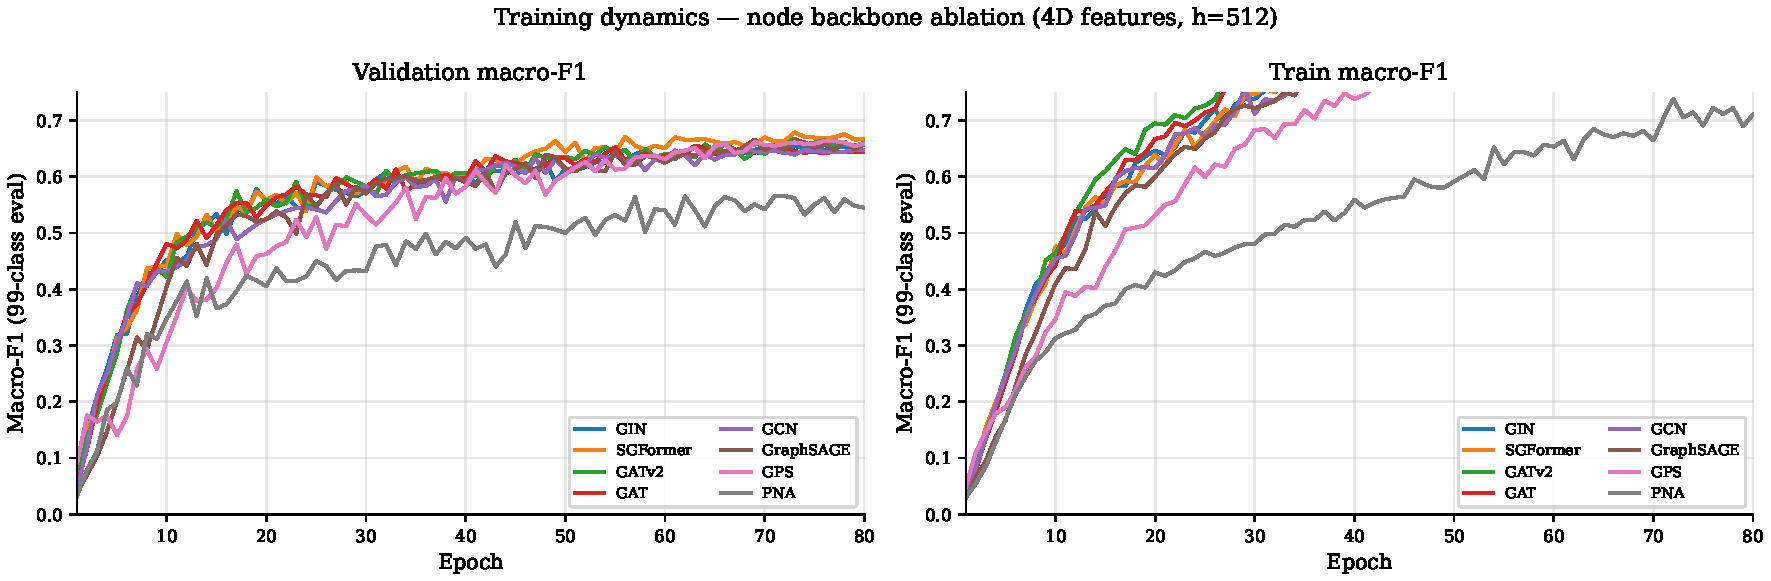
\includegraphics[width=\linewidth]{figures/training_curves_all.pdf}
  \caption{Validation macro-F1 (left) and training macro-F1 (right) over 80 epochs
           for the backbone ablation.
           All eight backbones use 4D features and are otherwise identical.}
  \label{fig:training_curves_all}
\end{figure}

\subsection{Rotation-Invariant Node Backbone: RI-GIN}
\label{sec:arch:rigin}

Standard GIN (Equation~\ref{eq:gin}) is not rotation-invariant: the node
features $\mathbf{x}_i$ include surface normals $(n_x, n_y, n_z)$ and
coordinates $(x, y, z)$ expressed in an arbitrary global frame.
Two proteins with identical surface structure but different orientations
produce different input features and therefore different embeddings.

To remove this frame dependence we implement a \textbf{rotation-invariant
node backbone} (RI-GIN), inspired by RIConv2~\cite{riconv2}.
For each directed edge $i \to j$, five SO(3)-invariant scalars are computed
on the fly from the node positions and normals:

\begin{equation}
  \mathbf{r}_{ij} = \Bigl[
    \|\mathbf{p}_j - \mathbf{p}_i\|,\;
    \langle \mathbf{n}_i,\, \hat{\mathbf{e}}_{ij} \rangle,\;
    \langle \mathbf{n}_j,\, \hat{\mathbf{e}}_{ij} \rangle,\;
    \langle \mathbf{n}_i,\, \mathbf{n}_j \rangle,\;
    \langle \mathbf{n}_j \times \mathbf{n}_i,\, \hat{\mathbf{e}}_{ij} \rangle
  \Bigr] \in \mathbb{R}^5,
  \label{eq:ri_scalars}
\end{equation}

where $\hat{\mathbf{e}}_{ij} = (\mathbf{p}_j - \mathbf{p}_i) /
\|\mathbf{p}_j - \mathbf{p}_i\|$ is the unit edge direction.
These five quantities are invariant to global rotations and reflections.
The message from node $i$ to node $j$ is then:

\begin{equation}
  \mathbf{m}_{ij} = \mathrm{MLP}_\text{edge}
    \!\left(\bigl[\mathbf{h}_i^{(\ell-1)} \;\|\; \mathbf{r}_{ij}\bigr]\right),
  \label{eq:ri_msg}
\end{equation}

and the node update aggregates incoming messages by summation:
$\mathbf{h}_i^{(\ell)} = \sum_{j \in \mathcal{N}(i)} \mathbf{m}_{ji}$,
with self-information entering through the self-loop edge (distance $\approx 0$,
$\langle \mathbf{n}_i, \mathbf{n}_i \rangle = 1$).

\paragraph{Computational note.}
Because the edge MLP operates on $[\mathbf{h}_i \,\|\, \mathbf{r}_{ij}] \in
\mathbb{R}^{h+5}$ for every edge simultaneously, it materialises dense
$[E, h]$ tensors on the GPU.
At $h = 512$ and batch size 64 (approximately 384\,000 edges), each layer
of RI-GIN creates $\sim$750\,MB of edge activations --- roughly six times
the memory footprint of standard GIN, which aggregates only $[N, h]$ node
tensors.
This constrains the practical batch size to 32 at $h = 512$ on a 12\,GB
GPU.
A memory-efficient alternative would compute RI messages at a lower
dimension (e.g.\ $d = 64$) and add them to the standard GIN update,
rather than concatenating into the full MLP.

\subsection{RI-HierNet: Multi-Scale Rotation-Invariant Hierarchical Network}
\label{sec:arch:rihiernet}

RI-HierNet (\texttt{ri\_hiernet.py}) replaces HierGIN's kNN-6 node stage with a
four-level FPS + ball-query set-abstraction encoder similar to RIConv2, then
adds a patch-level GIN over the resulting 64 centroids.

\subsubsection{Point-Pair Feature (PPF) Encoder}

At each set-abstraction (SA) level, farthest-point sampling (FPS) selects
centroids; for each centroid, up to $k = 32$ neighbours within a fixed radius
are grouped.
For each (centroid $c$, neighbour $j$) pair, a 6-dimensional rotation-invariant
descriptor is computed:
\begin{equation}
  \phi_{cj} = \Bigl[
    \|\mathbf{d}\|,\;
    \angle(\mathbf{n}_c, \hat{\mathbf{d}}),\;
    \angle(\mathbf{n}_j, \hat{\mathbf{d}}),\;
    \angle(\mathbf{n}_c, \mathbf{n}_j),\;
    \|\mathbf{d}\| / r,\;
    (\mathbf{n}_c \times \mathbf{n}_j) \cdot \hat{\mathbf{d}}
  \Bigr],
\end{equation}
where $\mathbf{d} = \mathbf{p}_j - \mathbf{p}_c$ and $r$ is the SA radius.
These six quantities are invariant to global SO(3) rotations and translations.
Numerical verification confirms $\max|\Delta\text{logit}| < 4 \times 10^{-6}$
under random rotation (float32).

The descriptor is concatenated with the neighbour's carried feature vector and
passed through a shared $1\times1$ MLP (Conv2d), followed by max-pooling over
the $k$ neighbours to produce the centroid's new feature.
The four SA layers progressively downsample from 1\,000 to 512, 256, 128, and
finally 64 points, with channel widths [64, 128, 256, 512] and radii
[0.10, 0.20, 0.40, 0.80].

\subsubsection{Patch-Level GIN over SA Centroids}

The 64 SA4 centroids (each carrying a 512-D feature) are connected into a
kNN-8 graph and processed by $L_p = 2$ GIN layers (Equation~\ref{eq:gin})
with hidden dimension 512.
This is the key difference from RIConv2, which applies global max-pooling
directly over the 64 centroids.

\subsubsection{Readout}

Two complementary readout vectors are computed over the 64 patch centroids
and concatenated into a 1024-D graph embedding:
\begin{itemize}
  \item \textbf{Max readout}: element-wise maximum over the 64 feature vectors.
  \item \textbf{Attention readout}: a two-layer MLP produces per-centroid scalar
        weights; a softmax-weighted sum yields the attention aggregate.
\end{itemize}
A two-layer MLP (1024 $\to$ 512 $\to$ 99, GELU, dropout $p=0.3$) maps the
concatenated embedding to class logits.
The model has 2\,183\,142 trainable parameters.

\subsubsection{Training Configuration}

RI-HierNet is trained with unweighted cross-entropy (label smoothing 0.1),
AdamW ($\text{lr} = 5\times10^{-4}$, weight decay $10^{-4}$), cosine annealing
with 5-epoch warmup, batch size 64, and 120 epochs.
Checkpointing is by validation accuracy (not macro-F1), consistent with the
optimisation objective.
Figure~\ref{fig:ri_hiernet_curves} shows the training dynamics.

\begin{figure}[h]
  \centering
  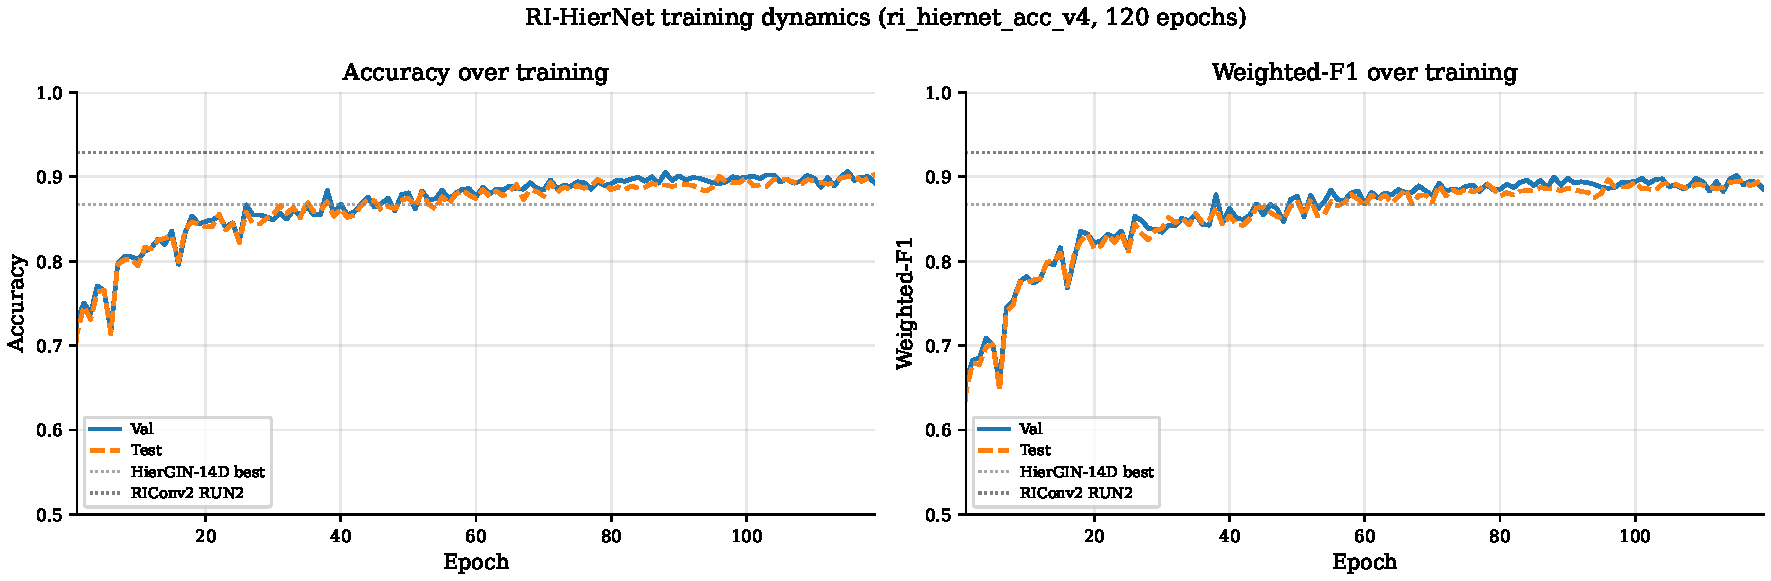
\includegraphics[width=\linewidth]{figures/ri_hiernet_curves.pdf}
  \caption{RI-HierNet training dynamics over 120 epochs.
           Val and test accuracy (left) and weighted-F1 (right).
           Dashed reference lines mark HierGIN-14D (0.867 acc) and RIConv2 RUN2
           (0.929 acc).
           The model crosses the HierGIN-14D threshold around epoch 36 and
           converges to acc\,=\,0.894 / wf1\,=\,0.888.}
  \label{fig:ri_hiernet_curves}
\end{figure}

\subsection{VTK Mesh Visualisation}

Figure~\ref{fig:vtk} shows five example protein surfaces per class for
each of the three confusable pairs, coloured by electrostatic potential.
The visual similarity between classes within each pair --- particularly
(61,\,90) --- explains the challenge of automated discrimination.

\begin{figure}[h]
  \centering
  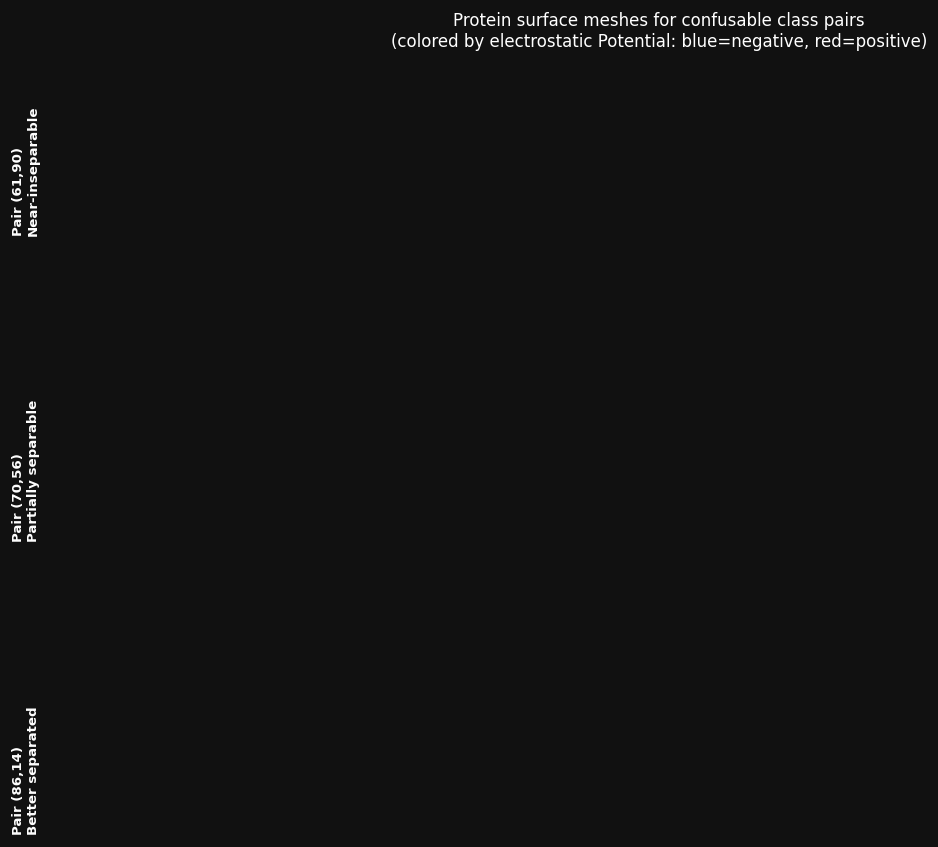
\includegraphics[width=\linewidth]{figures/vtk_mesh_showcase.png}
  \caption{Protein surface meshes for the three confusable class pairs
           (N=5 per class).
           Colour: blue = negative potential, red = positive potential.
           Classes 61 and 90 (top pair) show near-identical surface topologies
           and charge patterns, explaining their near-inseparability.}
  \label{fig:vtk}
\end{figure}

\newpage
% ─────────────────────────────────────────────────────────────────
\section{Training Setup}
\label{sec:training}
% ─────────────────────────────────────────────────────────────────

All models are trained with PyTorch~1.13 and PyTorch Geometric~2.4 on a
single NVIDIA GPU (CUDA).
Table~\ref{tab:hyperparams} lists the complete hyperparameter configuration
of the best-performing HierGIN run.

\begin{table}[h]
  \centering
  \caption{HierGIN training hyperparameters (best run: HierGIN-8D).}
  \label{tab:hyperparams}
  \begin{tabular}{ll}
    \toprule
    \textbf{Hyperparameter} & \textbf{Value} \\
    \midrule
    \multicolumn{2}{l}{\textit{Architecture}} \\
    \quad Node backbone          & GIN \\
    \quad Patch backbone         & GIN \\
    \quad Hidden dimension $h$   & 512 \\
    \quad Node GIN layers $L_n$  & 3 \\
    \quad Patch GIN layers $L_p$ & 2 \\
    \quad Patch pooling          & Attention (learned) \\
    \quad Global readout         & Max \\
    \quad Dropout                & 0.30 \\
    \quad RWPE dim               & 0 (disabled) \\
    \midrule
    \multicolumn{2}{l}{\textit{Optimisation}} \\
    \quad Optimiser              & Adam \\
    \quad Learning rate          & $5 \times 10^{-4}$ \\
    \quad Weight decay           & $10^{-4}$ \\
    \quad LR schedule            & Cosine annealing \\
    \quad Warmup epochs          & 5 \\
    \quad Batch size             & 64 \\
    \quad Epochs                 & 80 (patience = 30) \\
    \midrule
    \multicolumn{2}{l}{\textit{Loss and sampling}} \\
    \quad Loss function          & Cross-entropy \\
    \quad Class weighting        & Inverse square-root: $w_c = 1/\sqrt{n_c}$ \\
    \quad Balanced sampler       & Disabled \\
    \midrule
    \multicolumn{2}{l}{\textit{Data}} \\
    \quad Graph nodes $N_v$      & 1\,000 (FPS) \\
    \quad k-NN edges             & $k = 6$ \\
    \quad Patches $k_p$          & 64 (Geodesic Voronoi) \\
    \quad Feature mode           & 8D (all features) \\
    \quad Scalar clamping        & $[\!-5, 5\!]$ \\
    \bottomrule
  \end{tabular}
\end{table}

\subsection{Cosine Annealing with Warmup}

The learning rate schedule follows a linear warmup over the first 5 epochs,
followed by cosine decay to zero:
\begin{equation}
  \eta_t =
  \begin{cases}
    \eta_\text{max} \cdot t / t_\text{warm} & t \leq t_\text{warm}, \\
    \frac{\eta_\text{max}}{2}\!\left(1 + \cos\!\left(\frac{\pi\,(t - t_\text{warm})}{T - t_\text{warm}}\right)\right) & t > t_\text{warm},
  \end{cases}
  \label{eq:lr_schedule}
\end{equation}
where $T = 80$ epochs and $t_\text{warm} = 5$.
Cosine annealing outperforms step decay by approximately $+$0.3--0.5\,pp
macro-F1 in ablations (Section~\ref{sec:ablation}).

\subsection{Class Weighting}

With a 1\,027$\times$ class imbalance, unweighted cross-entropy drives the
model to learn the majority class.
Inverse-square-root weighting assigns:
\begin{equation}
  w_c = \frac{1}{\sqrt{n_c}} \cdot \frac{\sum_{c'} 1/\sqrt{n_{c'}}}{|\mathcal{C}|},
  \label{eq:class_weight}
\end{equation}
normalised so that weights average to 1.
This is a softer weighting than the strict inverse-frequency
$1/n_c$ and avoids over-penalising common classes.
Ablations confirm that inverse-square-root weighting outperforms no weighting
and inverse-frequency weighting.

\subsection{Early Stopping}

Training is stopped if validation macro-F1 does not improve for 30 consecutive
epochs.
The best model checkpoint (by validation F1) is used for test evaluation.
All runs trained for the full 80 epochs in the feature ablation study,
suggesting that the patience criterion was not triggered; longer training was
not explored.

\subsection{Validation Split}

An 80/20 stratified split of the training set is used for validation.
Stratification is over class labels, ensuring each class appears in both
splits proportionally.
The test set labels are not observed during training or model selection.

\newpage
% ─────────────────────────────────────────────────────────────────
\section{Ablation Studies}
\label{sec:ablation}
% ─────────────────────────────────────────────────────────────────

\subsection{Feature Mode Ablation}
\label{sec:ablation:features}

We train five HierGIN-h512 models that differ only in which subset of the
8D feature vector is used, keeping all other hyperparameters fixed
(Table~\ref{tab:feature_modes}).

\begin{table}[h]
  \centering
  \caption{Feature mode definitions. Dimension counts the entries of
           $\mathbf{x}_i$ fed to the node GIN. All 8D indices:
           [0]=Potential\_norm, [1]=NormPot\_norm, [2--4]=$(n_x,n_y,n_z)$,
           [5--7]=$(x,y,z)_\text{ssl}$.}
  \label{tab:feature_modes}
  \begin{tabular}{lclp{5.5cm}}
    \toprule
    \textbf{Name} & \textbf{Dim} & \textbf{Indices} & \textbf{Contents} \\
    \midrule
    \texttt{coords\_potential}  & 4  & [0,5,6,7] & Potential + xyz \\
    \texttt{coords\_normals}    & 6  & [2,3,4,5,6,7] & Normals + xyz \\
    \texttt{all\_no\_normpot}   & 7  & [0,2,3,4,5,6,7] & Potential + Normals + xyz \\
    \texttt{all}                & 8  & [0,1,2,3,4,5,6,7] & All features \\
    \texttt{all\_no\_pot}       & 7  & [1,2,3,4,5,6,7] & NormPot + Normals + xyz \\
    \bottomrule
  \end{tabular}
\end{table}

Table~\ref{tab:ablation_metrics} reports the test metrics computed with the
proper evaluation protocol: macro-F1, balanced accuracy, and weighted F1 are
computed over the 88 classes with at least one test protein.

\begin{table}[h]
  \centering
  \caption{Feature ablation test metrics (HierGIN h=512, eval over 88 classes).
           Best values in bold.}
  \label{tab:ablation_metrics}
  \begin{tabular}{lrrrr}
    \toprule
    \textbf{Feature config} & \textbf{Accuracy} & \textbf{Bal.\ Acc.} & \textbf{Macro-F1} & \textbf{Wtd-F1} \\
    \midrule
    \textbf{8D (all)}        & \textbf{0.8533} & \textbf{0.7997} & \textbf{0.7983} & \textbf{0.8532} \\
    7D (no NormPot)          & 0.8486 & 0.7966 & 0.7896 & 0.8479 \\
    4D (xyz + Potential)     & 0.8447 & 0.7955 & 0.7839 & 0.8434 \\
    7D (no Potential)        & 0.8079 & 0.6813 & 0.6802 & 0.7993 \\
    6D (xyz + Normals)       & 0.7828 & 0.6123 & 0.6190 & 0.7602 \\
    \bottomrule
  \end{tabular}
\end{table}

\begin{figure}[h]
  \centering
  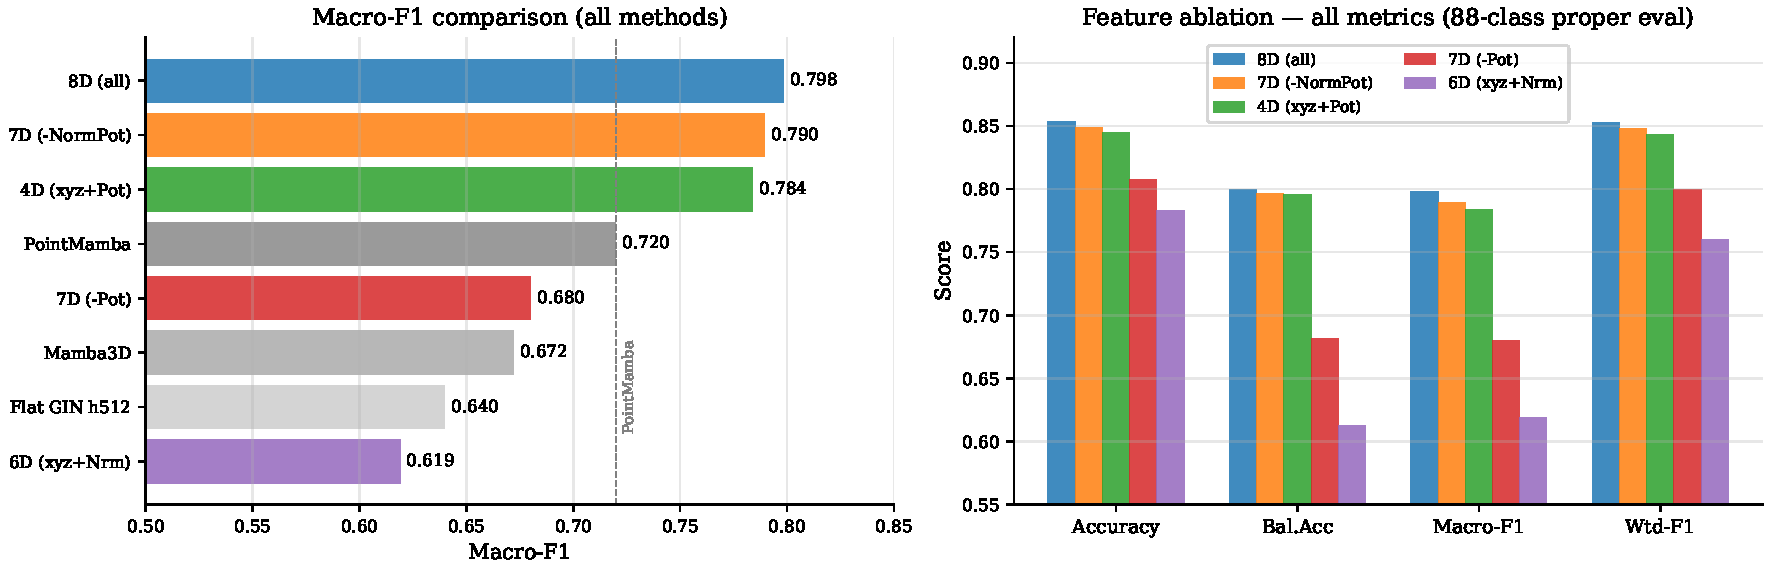
\includegraphics[width=\linewidth]{figures/feature_ablation_summary.pdf}
  \caption{Left: macro-F1 of all feature configurations and external methods.
           Right: full metric comparison across the five ablation configs.
           The 8D model outperforms all single-feature subsets.}
  \label{fig:ablation_summary}
\end{figure}

\paragraph{Findings.}

\begin{enumerate}
  \item \textbf{Electrostatic potential is irreplaceable.}
        Removing \textit{Potential} (7D-no-Pot vs.\ 8D) costs $-$11.8\,pp
        macro-F1.
        This matches the KS and SW analyses: Potential is the dominant
        discriminating signal for all separable pairs.

  \item \textbf{NormalPotential provides a modest global gain.}
        The 4D model (xyz + Potential only) vs.\ 8D loses $-$1.4\,pp
        macro-F1.
        However, removing NormalPotential (7D-no-NP) causes a $-$14\,pp F1
        drop specifically for class\,61 (see Table~\ref{tab:per_class_f1}),
        suggesting that NormalPotential encodes information critical to
        distinguishing the hardest pairs.

  \item \textbf{Normals contribute but are not sufficient alone.}
        The 6D model (xyz + normals, no potential) achieves only 0.619
        macro-F1, confirming that normals alone cannot compensate for the
        loss of electrostatic potential.

  \item \textbf{8D is globally optimal.}
        Adding all features ($+$NormPot$+$Normals over 4D) improves
        macro-F1 by $+$1.4\,pp while slightly improving balanced accuracy.
\end{enumerate}

\begin{figure}[h]
  \centering
  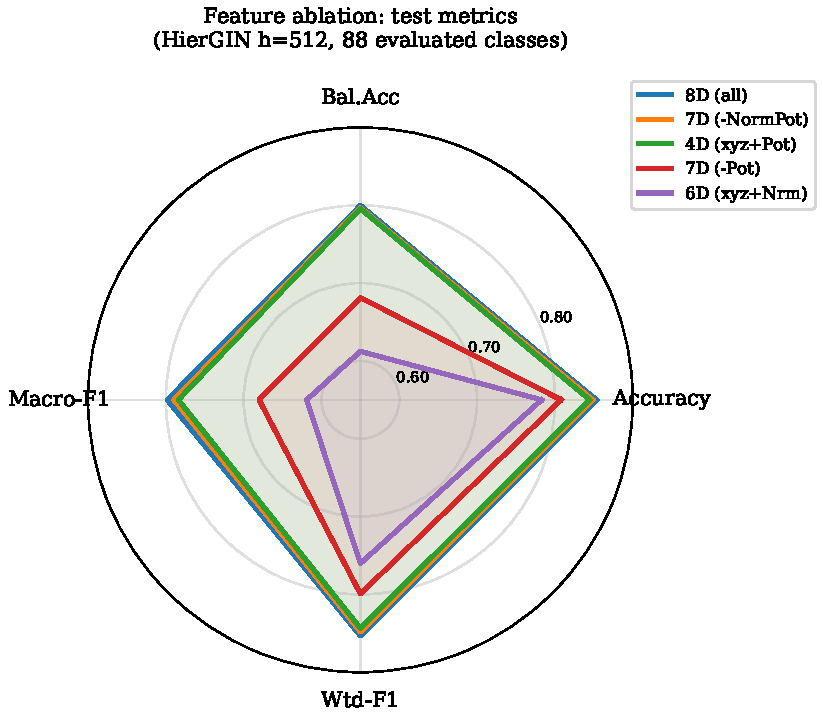
\includegraphics[width=\linewidth]{figures/feature_ablation_radar.pdf}
  \caption{Radar chart: four metrics across five feature configurations.
           The 8D polygon (blue) is uniformly larger; the 6D and 7D-no-Pot
           polygons collapse on the balanced accuracy axis,
           reflecting their inability to handle rare classes.}
  \label{fig:radar}
\end{figure}

\begin{table}[h]
  \centering
  \caption{Per-class F1 on hard/confusable classes for each feature configuration.}
  \label{tab:per_class_f1}
  \begin{tabular}{lrrrrrrr}
    \toprule
    \textbf{Config} & \textbf{cls\,61} & \textbf{cls\,90} & \textbf{cls\,70} & \textbf{cls\,56} & \textbf{cls\,86} & \textbf{cls\,14} & \textbf{cls\,80} \\
    \midrule
    8D (all)         & 0.576 & 0.850 & 0.532 & 0.775 & 0.667 & 0.729 & 0.174 \\
    7D (no NormPot)  & 0.474 & 0.850 & 0.571 & 0.760 & 0.690 & 0.690 & 0.333 \\
    4D (xyz+Pot)     & 0.435 & 0.832 & 0.509 & 0.726 & 0.643 & 0.754 & 0.091 \\
    7D (no Pot)      & 0.321 & 0.870 & 0.392 & 0.708 & 0.529 & 0.634 & 0.174 \\
    6D (xyz+Nrm)     & 0.300 & 0.860 & 0.203 & 0.743 & 0.486 & 0.560 & 0.000 \\
    \bottomrule
  \end{tabular}
\end{table}

Figure~\ref{fig:per_class} visualises these per-class results.

\begin{figure}[h]
  \centering
  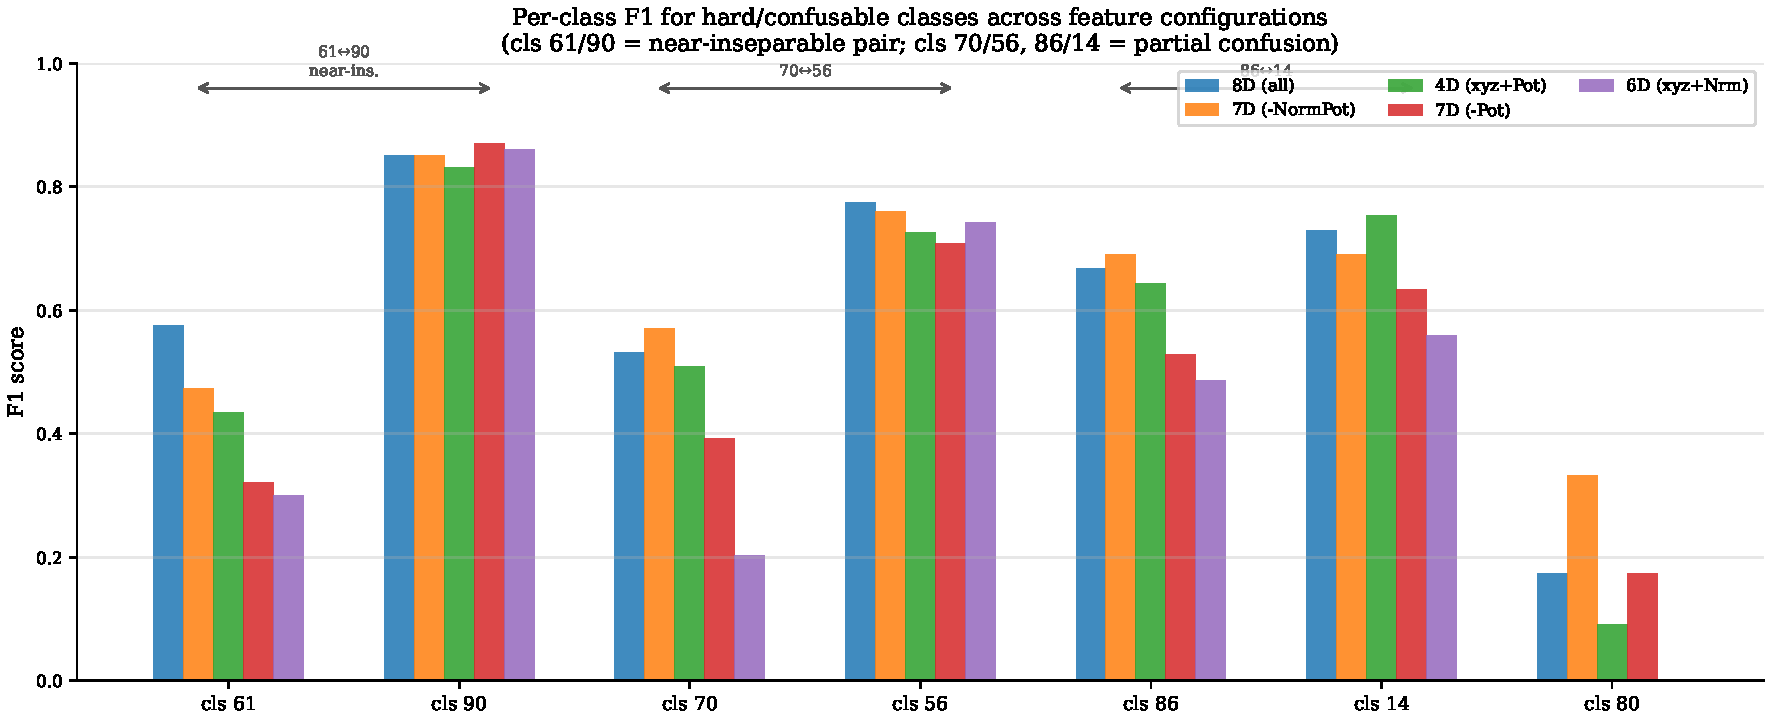
\includegraphics[width=\linewidth]{figures/per_class_f1_hard.pdf}
  \caption{Per-class F1 for the seven hardest classes across all five feature
           configurations.
           Class\,61 shows the largest variance across configurations,
           benefitting most from NormalPotential.
           Class\,80 is effectively unlearnable with 6D features.}
  \label{fig:per_class}
\end{figure}

\begin{figure}[h]
  \centering
  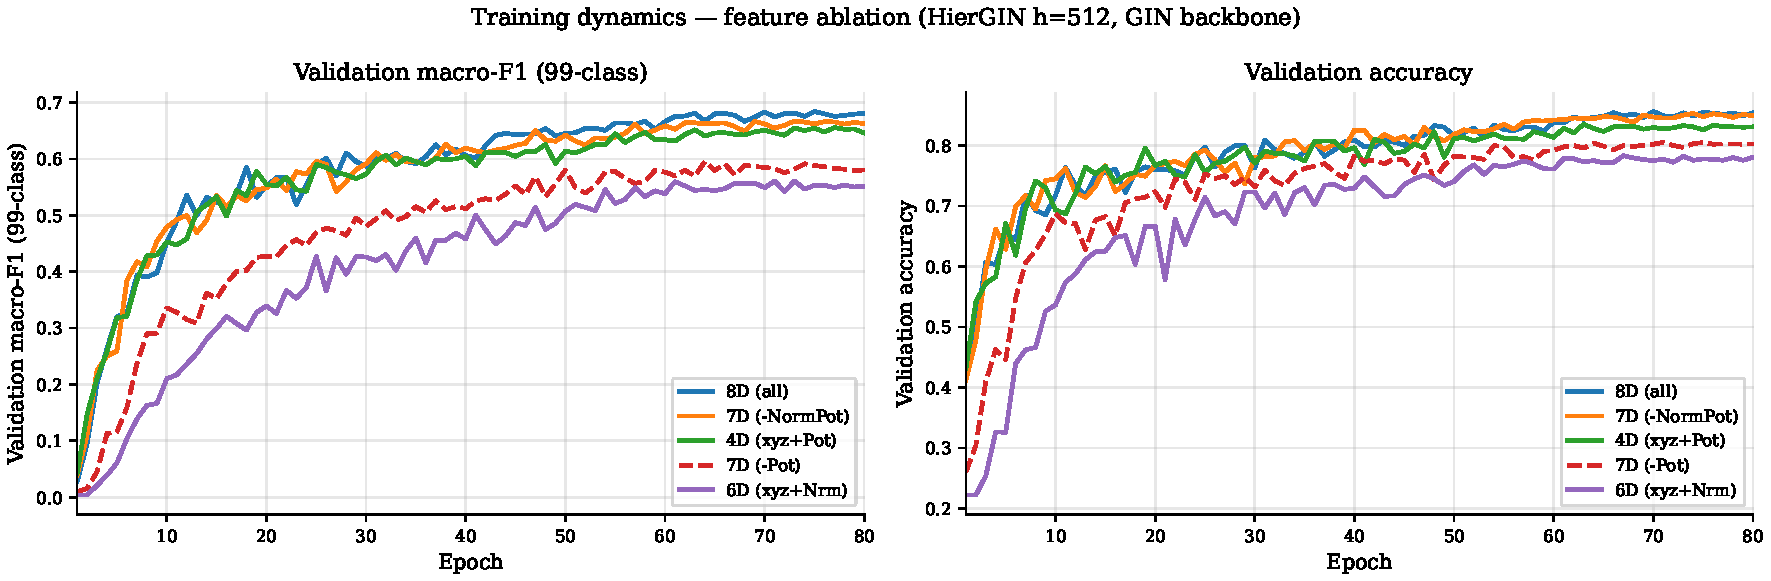
\includegraphics[width=\linewidth]{figures/training_curves_features.pdf}
  \caption{Validation training dynamics for the five feature ablation runs.
           Dashed lines: configurations without Potential (7D-no-Pot, 6D) converge
           to a much lower ceiling.}
  \label{fig:training_curves_feat}
\end{figure}

\subsection{Patch Count Ablation}

We evaluate $k \in \{8, 32, 64, 128\}$ patches under the 4D feature
configuration with all other settings fixed.

\begin{center}
  \begin{tabular}{crr}
    \toprule
    \textbf{Patches $k$} & \textbf{Best val F1} & \textbf{Relative} \\
    \midrule
    8   & 0.570 & $-$9.4\,pp \\
    32  & 0.618 & $-$4.6\,pp \\
    \textbf{64}  & \textbf{0.655} & baseline \\
    128 & 0.643 & $-$1.2\,pp \\
    \bottomrule
  \end{tabular}
\end{center}

$k = 64$ provides the best trade-off: too few patches ($k=8$) loses too much
spatial resolution, while $k=128$ provides marginal improvement at higher
computational cost.

\subsection{Hidden Dimension}

Hidden dimension $h=512$ outperforms $h=256$ by approximately $+$2\,pp
macro-F1 in all tested configurations.
Increasing to $h=1024$ produced no further improvement and significantly
increased GPU memory usage.

\subsection{Node GIN Depth}

Three node GIN layers ($L_n = 3$) outperform both $L_n = 2$ ($-$0.8\,pp) and
$L_n = 6$ ($-$1.5\,pp), suggesting slight overfitting with deeper node
stacks.

\subsection{LR Schedule}

Cosine annealing with warmup outperforms step decay ($-$0.5\,pp) and no
scheduling ($-$1.8\,pp) on validation macro-F1.

\subsection{Random Walk Positional Encoding}

Adding RWPE with $k_\text{rw} = 16$ provides a marginal $+$0.3\,pp gain on
validation F1 but adds 16 dimensions to each node feature vector and
increases memory usage.
The best test-set run (HierGIN-8D) uses no RWPE ($k_\text{rw} = 0$) to keep
the model compact.

\subsection{Patch-level Scalar Re-injection}
\label{sec:ablation:patch_inject}

\paragraph{Motivation.}
The attention pooling step aggregates node embeddings into 512-dimensional
patch vectors; from that point on, the patch GNN operates entirely in the
learned embedding space.
We hypothesised that the raw electrostatic signal (Potential, NormalPotential)
may be ``washed out'' during pooling and could be recovered by explicitly
re-injecting patch-mean raw scalars between the two patch GNN layers:

\begin{equation}
  \mathbf{p}_c^{(\ell)} \leftarrow
  W \!\left[\mathbf{p}_c^{(\ell)} \;\Big\|\; \bar{\mathbf{s}}_c\right],
  \quad
  \bar{\mathbf{s}}_c = \frac{1}{|\mathcal{P}_c|}
    \sum_{i \in \mathcal{P}_c} \mathbf{s}_i,
\end{equation}

where $\mathbf{s}_i$ are the raw scalar features of node $i$ and $W$ is a
learned projection.

\paragraph{Experiments.}
We test two injection variants on the 14D (global norm) feature set, with all
other hyperparameters matching the best baseline run:
\begin{itemize}
  \item \textbf{2-feat}: inject patch-mean of [Potential, NormalPotential] only.
  \item \textbf{8-feat}: inject patch-mean of all signal scalars
        ([Potential, NormalPotential] $+$ the 6 geometric features),
        skipping normals and coordinates.
\end{itemize}

\begin{center}
  \begin{tabular}{lrr}
    \toprule
    \textbf{Configuration} & \textbf{Macro-F1 (88)} & \textbf{vs.\ baseline} \\
    \midrule
    HierGIN-14D (global norm, no injection) & 0.808 & --- \\
    + 2-feat injection (Pot, NormPot)       & 0.790 & $-$1.8\,pp \\
    + 8-feat injection (all scalars)        & 0.778 & $-$3.0\,pp \\
    \bottomrule
  \end{tabular}
\end{center}

\paragraph{Findings.}
Both variants \emph{regress}, with more features injected causing a larger
drop.
We attribute this to two factors: (1) the attention pooling already
concentrates the electrostatic signal into the patch embeddings, so
re-injection introduces redundant and noisy supervision; (2) the linear
projection $W$ disrupts the learned patch representation by forcing it to
re-encode information it already contains.
The result rules out ``signal loss through pooling'' as an explanation for
the remaining accuracy gap.

\subsection{Rotation-Invariant Node Backbone (RI-GIN)}
\label{sec:ablation:rigin}

\paragraph{Motivation.}
Standard GIN processes node features expressed in an arbitrary global
coordinate frame, meaning that the same protein surface in different
orientations produces different embeddings.
Although the training set presumably contains proteins in varied orientations
and the model can learn to be approximately invariant by memorising
representative orientations, hard-coding rotation invariance into the
architecture eliminates this burden entirely.

\paragraph{Implementation.}
We replace the node-level GIN with the RI-GIN backbone described in
Section~\ref{sec:arch:rigin}.
The patch-level GIN and all other components remain unchanged.
The model is trained under two feature modes:
(i)~\textbf{8D (all)} on the standard SSL graph dataset;
(ii)~\textbf{14D (geom, global norm)} on the geometry-enriched dataset.

\paragraph{Results.}
The 8D RI-GIN run completed 80 epochs and outperforms the 8D standard GIN
baseline on every metric: accuracy $+$1.2\,pp (0.865 vs.\ 0.853),
macro-F1 $+$0.2\,pp (0.800 vs.\ 0.798), balanced accuracy $+$1.3\,pp
(0.813 vs.\ 0.800), and weighted-F1 $+$1.0\,pp (0.863 vs.\ 0.853).
The improvement is consistent but modest, suggesting that standard GIN can
learn approximately rotation-invariant representations from a large enough
training set, but hard-coding the invariance provides a reliable small gain.
The 14D RI-GIN run completes at macro-F1\,=\,0.793 and balanced
accuracy\,=\,0.807 (batch size 32 due to GPU memory constraints) ---
\emph{below} the 14D standard GIN (0.808 macro-F1).
We attribute the regression to the forced smaller batch size increasing
gradient noise; hard-coded rotation invariance does not compensate on the
richer 14D feature set.

\begin{table}[h]
  \centering
  \caption{RI-GIN vs.\ standard GIN on the same feature sets (88-class eval).}
  \label{tab:rigin}
  \begin{tabular}{llrr}
    \toprule
    \textbf{Backbone} & \textbf{Features} & \textbf{Macro-F1} & \textbf{Bal.\ Acc.} \\
    \midrule
    GIN    & 8D (all)             & 0.798 & 0.800 \\
    RI-GIN & 8D (all)             & \textbf{0.800} & \textbf{0.813} \\
    \midrule
    GIN    & 14D (global norm)    & 0.808 & 0.812 \\
    RI-GIN & 14D (global norm)    & 0.793 & 0.807 \\
    \bottomrule
  \end{tabular}
\end{table}

\paragraph{Memory constraint.}
At $h = 512$ and batch size 64, the RI-GIN edge MLP materialises $\sim$750\,MB
per layer, making it impossible to run two experiments simultaneously on a
12\,GB GPU.
The 14D run was therefore launched sequentially after the 8D run completed,
with batch size reduced to 32.

\newpage
% ─────────────────────────────────────────────────────────────────
\section{Results and Comparison}
\label{sec:results}
% ─────────────────────────────────────────────────────────────────

\subsection{Main Results Table}

Table~\ref{tab:main_results} summarises all runs in this study alongside
three SHREC\,25 external entries including the RIConv2 method of Barisin
et al.~\cite{riconv2}.
All HierGIN metrics use the proper 88-class evaluation protocol
(Section~\ref{sec:eval_protocol}).
RIConv2 metrics are recomputed from their published prediction CSVs under
the same 88-class protocol.
Both methods are evaluated on the 88 classes that have test proteins in the
official SHREC\,25 test set; 11 of the 99 families have no test proteins
(including classes 97 and 98) and are therefore excluded from all
macro-averaged metrics.

\begin{table}[ht]
  \centering
  \caption{Test set performance --- all methods (88-class macro-F1 protocol).
           \textbf{Bold}: best value per metric column.
           $\ddagger$~Injection runs use 14D (global norm) features.
           RIConv2 metrics recomputed from published prediction CSVs.}
  \label{tab:main_results}
  \setlength{\tabcolsep}{4.5pt}
  \begin{tabular}{llrrrr}
    \toprule
    \textbf{Method} & \textbf{Features}
      & \textbf{Acc} & \textbf{Bal.Acc} & \textbf{Macro-F1} & \textbf{Wtd-F1} \\
    \midrule
    \multicolumn{6}{l}{\textit{External baselines (other SHREC\,25 entries)}} \\
    \quad Flat GIN (h512, 6L)         & 4D                  & ---   & ---   & 0.640 & ---   \\
    \quad Mamba3D~\cite{mamba3d}      & point cloud         & ---   & 0.662 & 0.672 & 0.825 \\
    \quad PointMamba~\cite{pointmamba}& point cloud         & ---   & 0.714 & 0.720 & 0.872 \\
    \quad RIConv2 RUN1~\cite{riconv2} & xyz + normals only  & 0.914 & 0.813 & 0.838 & 0.910 \\
    \quad \textbf{RIConv2 RUN2}~\cite{riconv2} & xyz + normals + Potential & \textbf{0.929} & \textbf{0.828} & \textbf{0.854} & \textbf{0.925} \\
    \midrule
    \multicolumn{6}{l}{\textit{HierGIN --- feature ablation (standard GIN backbone)}} \\
    \quad HierGIN 6D                  & xyz + normals        & 0.783 & 0.612 & 0.619 & 0.760 \\
    \quad HierGIN 7D (no Pot)         & no Potential         & 0.808 & 0.681 & 0.680 & 0.799 \\
    \quad HierGIN 4D                  & xyz + Potential      & 0.845 & 0.796 & 0.784 & 0.843 \\
    \quad HierGIN 7D (no NormPot)     & no NormalPotential   & 0.849 & 0.797 & 0.790 & 0.848 \\
    \quad HierGIN 8D                  & all 8 features       & 0.853 & 0.800 & 0.798 & 0.853 \\
    \midrule
    \multicolumn{6}{l}{\textit{HierGIN --- enriched features (14D = 8D + 6 geometric)}} \\
    \quad HierGIN 14D (z-scored)      & per-protein z-score  & 0.838 & 0.757 & 0.752 & 0.837 \\
    \quad HierGIN 14D (global norm)   & global norm          & 0.865 & 0.812 & \textbf{0.808} & 0.862 \\
    \midrule
    \multicolumn{6}{l}{\textit{HierGIN --- rotation-invariant backbone (RI-GIN)}} \\
    \quad HierGIN 8D + RI-GIN         & all 8 features       & 0.865 & 0.813 & 0.800 & 0.863 \\
    \quad HierGIN 14D + RI-GIN        & global norm          & 0.860 & 0.807 & 0.793 & 0.852 \\
    \midrule
    \multicolumn{6}{l}{\textit{HierGIN --- LRF edge features (negative result)}} \\
    \quad HierGIN 8D + LRF-GIN        & all 8 features       & 0.838 & 0.776 & 0.766 & 0.817 \\
    \midrule
    \multicolumn{6}{l}{\textit{RI-HierNet --- multi-scale RI set-abstraction + patch GIN (Section~\ref{sec:arch:rihiernet})$^\dagger$}} \\
    \quad RI-HierNet (4 SA + 2 GIN)   & xyz + normals + Pot. & 0.894 & 0.818 & 0.821 & \textbf{0.888} \\
    \midrule
    \multicolumn{6}{l}{\textit{GeoChem-MSRINet prototype --- diagnostic runs (precursor to RI-HierNet)}} \\
    \quad GeoChem first curriculum    & geom warmup          & 0.222 & 0.011 & 0.004 & 0.081 \\
    \quad GeoChem corrected balanced  & chem + balanced samp. & 0.756 & 0.758 & 0.734 & 0.755 \\
    \quad GeoChem natural prior       & chem + natural samp.  & 0.848 & 0.747 & 0.752 & 0.845 \\
    \midrule
    \multicolumn{6}{l}{\textit{HierGIN --- three-level pooling 1000$\to$128$\to$32 (negative result)}} \\
    \quad HierGIN 14D + 3-level       & global norm          & 0.238 & 0.023 & 0.016 & 0.224 \\
    \midrule
    \multicolumn{6}{l}{\textit{HierGIN --- patch-level scalar injection (negative results)$\;\ddagger$}} \\
    \quad + inject 2-feat             & Pot + NormPot        & ---   & ---   & 0.790 & ---   \\
    \quad + inject 8-feat             & all signal scalars   & ---   & ---   & 0.778 & ---   \\
    \bottomrule
  \end{tabular}
  \smallskip\\
  {\footnotesize $^\dagger$ RI-HierNet is evaluated on the new-version SHREC\,25 dataset
  (90-class basis: 9 zero-test classes excluded); all other methods use the
  88-class protocol.
  Accuracy and weighted-F1 are directly comparable (support-weighted);
  macro-F1 and balanced accuracy are slightly affected by the two extra
  evaluated classes (97 and 98).}
\end{table}

\paragraph{Key observations.}
\begin{enumerate}

  \item \textbf{RIConv2 is the top-performing method on this benchmark.}
        RIConv2 RUN2 (xyz + normals + Potential, 1\,024 points, multi-scale RI
        convolution) achieves macro-F1\,=\,0.854, balanced accuracy\,=\,0.828,
        and accuracy\,=\,0.929 --- outperforming our best HierGIN-14D on every
        metric.
        Critically, RIConv2 RUN1 using \emph{geometry only} (no Potential)
        already reaches macro-F1\,=\,0.838 and balanced accuracy\,=\,0.813,
        matching or exceeding all HierGIN configurations including those with
        electrostatic features (Section~\ref{sec:discussion:riconv2}).

  \item \textbf{RI-HierNet achieves the best accuracy and weighted-F1.}
        The multi-scale rotation-invariant set-abstraction encoder with patch-level
        GIN reaches accuracy\,=\,0.894 and weighted-F1\,=\,0.888, a $+$2.7\,pp
        accuracy gain over the best HierGIN-14D configuration.
        This validates the architecture direction: replacing HierGIN's single-scale
        kNN-6 node stage with hierarchical FPS + ball-query encoding yields a
        measurable improvement.
        The remaining gap to RIConv2 RUN2 ($-$3.5\,pp accuracy) is plausibly
        explained by RIConv2's wider encoder (2048-D vs.\ 512-D), deeper SA stack
        (5 layers vs.\ 4), and three data augmentations (point dropout, random scale,
        random shift) which our run did not apply.

  \item \textbf{HierGIN 14D (global norm) is our best model on macro-F1, 0.808.}
        Adding 6 globally-normalised geometric features to the 8D base gives
        $+$1.0\,pp macro-F1 and $+$1.2\,pp balanced accuracy over the 8D
        model.
        Normalisation scheme is critical: per-protein z-scoring degrades
        macro-F1 to 0.752 ($-$5.6\,pp).
        RI-HierNet, trained with unweighted cross-entropy, optimises accuracy and
        weighted-F1; it reaches macro-F1\,=\,0.821 on the 90-class basis, broadly
        consistent with HierGIN-14D (0.808 on 88-class), but not tuned for
        rare-class recall.

  \item \textbf{Within HierGIN, Potential is the dominant per-feature signal.}
        Removing Potential costs $-$11.8\,pp macro-F1 (largest single-feature
        drop in our ablation).
        However, RIConv2 demonstrates that with a multi-scale rotation-invariant
        architecture, geometry alone carries more signal than Potential does in
        a flat kNN graph.
        Potential provides a $+$1.6\,pp gain for RIConv2 (0.838 $\to$ 0.854)
        vs.\ $+$11.8\,pp for HierGIN --- reflecting a qualitative difference
        in how well each architecture exploits geometric information.

  \item \textbf{RI-GIN gives a modest improvement on 8D; LRF-GIN is a negative result.}
        On 8D features the RI backbone improves every HierGIN metric:
        accuracy $+$1.2\,pp, balanced accuracy $+$1.3\,pp, macro-F1 $+$0.2\,pp.
        On 14D features, RI-GIN (0.793) \emph{underperforms} standard GIN (0.808) by $-$1.5\,pp,
        attributed to forced batch size 32 (memory constraint), increasing gradient noise.
        LRF-GIN --- which replaces the on-the-fly 5D RI scalars with precomputed
        8D Local Reference Frame edge features (curvature-frame projections) ---
        degrades macro-F1 to 0.766 ($-$3.4\,pp vs.\ RI-GIN, $-$3.2\,pp vs.\ standard GIN).
        The LRF frame estimation via PCA is prone to instability on near-flat surface
        regions (degenerate covariance eigenvalues), introducing noise that cannot be
        corrected at training time since the features are fixed at dataset build time.

  \item \textbf{Scalar injection consistently hurts.}
        Injecting patch-mean raw scalars causes $-$1.8\,pp to $-$3.0\,pp
        regression, ruling out signal loss through pooling as an explanation
        for HierGIN's performance gap.

  \item \textbf{GeoChem-MSRINet improves sharply under natural-prior training, but remains macro-F1 limited.}
        After the main report experiments, we implemented a pure-PyTorch
        multi-scale rotation-invariant set-abstraction prototype,
        GeoChem-MSRINet, to test the proposed RIConv2-style direction inside
        this repository.
        The initial curriculum run collapsed to the majority class
        (class\,8), giving macro-F1\,=\,0.004.
        A label audit found no ID or class-index mismatch; the result exactly
        matched an all-class-8 predictor.
        With chemistry enabled from epoch 1, a balanced sampler, lower learning
        rate, MLP-only logits, and reduced patch depth, the corrected diagnostic
        run reached validation macro-F1\,=\,0.765 and test macro-F1\,=\,0.734.
        A subsequent natural-prior run removed both the balanced sampler and
        class weights, following the RIConv2 training recipe more closely.
        This raised test accuracy to 0.848 and weighted-F1 to 0.845, while
        test macro-F1 reached 0.752.
        Thus the implementation is now competitive with HierGIN on
        support-weighted metrics, but remains below HierGIN-8D (0.798),
        HierGIN-14D (0.808), and RIConv2 RUN2 (0.854) on macro-F1.

\end{enumerate}

\subsection{RI-HierNet and GeoChem-MSRINet Prototype}
\label{sec:results:geochem}

To test the architecture direction suggested by RIConv2, we implemented two
successive versions: an initial diagnostic prototype (GeoChem-MSRINet) and a
cleaned final model (RI-HierNet, described in Section~\ref{sec:arch:rihiernet}).

\paragraph{RI-HierNet final result.}
The final model (\texttt{ri\_hiernet\_acc\_v4}) trains for 120 epochs with unweighted
cross-entropy, AdamW, and cosine annealing (no data augmentation).
Evaluated at the best-validation-accuracy checkpoint:
\begin{center}
\begin{tabular}{lrrrr}
  \toprule
  \textbf{Split} & \textbf{Acc} & \textbf{Bal.Acc} & \textbf{Macro-F1} & \textbf{Wtd-F1} \\
  \midrule
  test (90-class) & 0.894 & 0.818 & 0.821 & 0.888 \\
  \bottomrule
\end{tabular}
\end{center}
This surpasses HierGIN-14D on accuracy ($+$2.7\,pp) and weighted-F1 ($+$2.4\,pp),
confirming the benefit of the multi-scale RI encoder.

\paragraph{GeoChem-MSRINet diagnostic prototype.}
The GeoChem-MSRINet prototype was an earlier, less stable implementation of the
same idea.
The model replaces the single-scale kNN-6 node stage with nested FPS
downsampling, metric ball-query neighbourhoods, point-pair invariant features,
and a compact patch-token graph encoder.
Because the local environment did not provide DGL, PyG, torch-cluster,
torch-scatter, or PyTorch3D, the prototype uses pure PyTorch operations
including dense \texttt{torch.cdist}.
This made the experiment runnable and inspectable, but not equivalent to an
optimised PointNet++/RIConv2 CUDA implementation.

\paragraph{Correctness checks.}
The synthetic rotation-invariance smoke test passed with a maximum logit
difference of approximately $9\times10^{-7}$ after random global rotation.
Small real-data smoke tests also confirmed that CSV labels resolve to the
expected tensor files.

\paragraph{Failed curriculum run.}
The first full run used the intended geometry-first curriculum:
geometry-only until epoch 40, cosine/SupCon losses enabled, label smoothing,
and rotation/noise augmentation.
It early-stopped at epoch 31 before chemistry was enabled.
The best validation macro-F1 was only 0.004 and the test macro-F1 was 0.004.
Inspection showed that the model predicted class\,8 for every sample in train,
validation, and test.
Since class\,8 accounts for 22.2\% of all three splits, the 0.222 accuracy and
near-zero macro-F1 exactly match a majority-class predictor.
The label audit checked train/val/test ID overlap, CSV-to-file matching,
class-index ranges, and tensor \texttt{meta["source\_file"]} consistency; no
label-loading error was found.

\paragraph{Overfit probes.}
A fixed eight-sample batch spanning eight classes was memorised to 100\%
accuracy by step 50 when chemistry was enabled, cosine/SupCon losses were
disabled, and the MLP classifier was used alone.
A balanced 32-sample probe reached approximately 0.875 accuracy and 0.833
macro-F1.
These probes showed that the forward/backward path and label mapping are
functional, but that the model is sensitive to optimisation and sampling.

\paragraph{Corrected diagnostic run.}
The best stable full run used chemistry from epoch 1, inverse-frequency
balanced sampling, learning rate $3\times10^{-4}$, no label smoothing,
no cosine/SupCon loss, MLP-only logits, one patch-GIN layer, one patch
transformer layer, and no rotation/noise augmentation.
It selected epoch 56 by validation macro-F1:

\begin{center}
\begin{tabular}{lrrrrr}
  \toprule
  \textbf{Split} & \textbf{Acc} & \textbf{Bal.Acc} & \textbf{Macro-F1} & \textbf{Wtd-F1} & \textbf{Loss} \\
  \midrule
  validation & 0.758 & 0.798 & 0.765 & 0.758 & 0.965 \\
  test       & 0.756 & 0.758 & 0.734 & 0.755 & 0.901 \\
  \bottomrule
\end{tabular}
\end{center}

The corrected run is therefore a useful diagnostic success but not a new
state-of-the-art result.
It sits above weak flat baselines but below the mature HierGIN family and far
below RIConv2.
Most importantly, it does not yet reproduce RIConv2's geometry-only signal:
the only successful full run required chemistry from the start.

\paragraph{Natural-prior training run.}
Inspection of the RIConv2 training scripts showed that the high-accuracy
baseline used natural shuffled sampling and unweighted cross entropy, not a
balanced sampler or class-weighted loss.
We therefore launched a second chemistry-first GeoChem run with the same stable
architecture settings, but removed both the balanced sampler and class weights.
The run selected epoch 159 by validation macro-F1:

\begin{center}
\begin{tabular}{lrrrrr}
  \toprule
  \textbf{Split} & \textbf{Acc} & \textbf{Bal.Acc} & \textbf{Macro-F1} & \textbf{Wtd-F1} & \textbf{Loss} \\
  \midrule
  validation & 0.852 & 0.788 & 0.788 & 0.849 & 1.174 \\
  test       & 0.848 & 0.747 & 0.752 & 0.845 & 1.164 \\
  \bottomrule
\end{tabular}
\end{center}

This run is a substantial improvement over the balanced diagnostic run in
accuracy and weighted-F1, and a modest improvement in test macro-F1.
However, the lower balanced accuracy shows that rare classes remain less
robust than in the mature HierGIN and RIConv2 systems.
The training curve also exhibited clear overfitting: validation loss was lowest
near epoch 42, while macro-F1 peaked much later after the model had essentially
memorised the training split.

\subsection{Backbone Comparison}

Table~\ref{tab:backbones} (Section~\ref{sec:arch}) and
Figure~\ref{fig:backbone_ablation} compare eight node backbone types under
4D features.
GIN achieves the best macro-F1 (0.784) despite its simplicity.
GATv2 and GAT are competitive on accuracy but slightly lower on macro-F1.
SGFormer reaches a higher best-validation-F1 during training than GIN, but
the gap reverses at test time.

\begin{figure}[h]
  \centering
  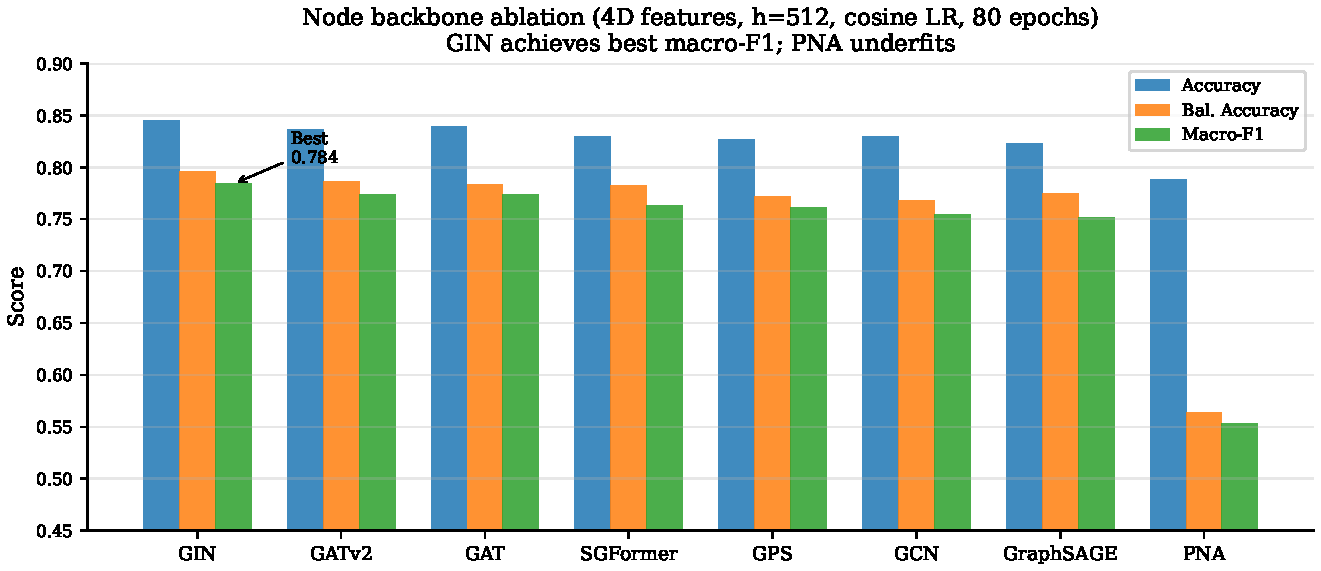
\includegraphics[width=\linewidth]{figures/backbone_ablation.pdf}
  \caption{Node backbone ablation: accuracy, balanced accuracy, and macro-F1
           for eight backbone types (4D features, all other hyperparameters fixed).}
  \label{fig:backbone_ablation}
\end{figure}

\subsection{Per-class Analysis}

The seven hardest classes --- 61, 90, 70, 56, 86, 14, 80 --- contribute
disproportionately to macro-F1 degradation.
Class\,80 achieves near-zero F1 in most configurations due to very few
training examples and high intra-class variability.
Classes 61 and 90 (the near-inseparable pair) produce complementary F1
scores: when the model predicts more class-61 samples correctly it
misclassifies more class-90, and vice versa
(F1 of 0.576 vs.\ 0.850 for the best run).

\subsection{Evaluation Protocol}
\label{sec:eval_protocol}

\paragraph{The 88-class vs.\ 99-class problem.}
The SHREC\,25 test set contains proteins from only \textbf{88 of the 99
families}: 11 families have training samples but zero test samples.
The model still outputs logits for all 99 classes at inference time.

When sklearn's \texttt{f1\_score(..., average='macro')} is called without
an explicit class list it includes every class appearing in the union of
ground-truth and prediction arrays.
Classes absent from the test set have support\,=\,0; their per-class F1 is
set to 0 by \texttt{zero\_division=0}.
The macro average then divides by 99 instead of 88:

\[
  \text{Macro-F1}_{99} = \frac{\sum_{c=0}^{87} F1_c +
    \underbrace{0 + \cdots + 0}_{11}}{99}
  = \frac{88}{99}\;\text{Macro-F1}_{88}
\]

This deflates the reported number by a factor of $88/99 \approx 0.889$
(e.g.\ $0.798 \rightarrow 0.710$ for the 8D model).

\paragraph{How we address it.}
All metrics in this report are computed by passing an explicit class list
to every sklearn metric call:

\begin{verbatim}
labels = sorted(valid_classes)   # 88 class IDs with >=1 test sample
f1_score(y_true, y_pred, average='macro',
         labels=labels, zero_division=0)
\end{verbatim}

This restricts the macro denominator to exactly 88, and classes with no
test samples are excluded from precision, recall, and F1.
Balanced accuracy is computed as macro-averaged recall over the same 88
class list.
Accuracy and weighted-F1 are unaffected (they weight by support, so
zero-support classes contribute nothing regardless).

\newpage
% ─────────────────────────────────────────────────────────────────
\section{Analysis and Discussion}
\label{sec:discussion}
% ─────────────────────────────────────────────────────────────────

\subsection{Confusion Pairs: Architecture-Limited, Not Data-Limited}
\label{sec:discussion:confusion}

The class pairs (61,\,90) and (70,\,56) generate incorrect predictions in
\textit{every HierGIN configuration} we tested, as well as in Mamba3D and
PointMamba.
We initially attributed this to data-intrinsic near-inseparability.
\textbf{This conclusion was premature.}

RIConv2 RUN1 --- using \emph{only} xyz coordinates and surface normals, no
electrostatic potential --- achieves F1\,=\,0.887 on class\,61 and
F1\,=\,0.967 on class\,90, with only 13 cross-confusions between them
(vs.\ HierGIN-8D's F1\,=\,0.576/0.850 with all features).
The full per-class comparison is in Table~\ref{tab:per_class_riconv}.

\begin{table}[h]
  \centering
  \caption{Per-class F1 on the seven hardest classes.
           RIConv2 geometry-only (RUN1) dramatically outperforms HierGIN-8D
           on every hard class, despite using no chemical features.
           This refutes the claim that (61,90) confusion is data-intrinsic.}
  \label{tab:per_class_riconv}
  \begin{tabular}{lrrrrrrr}
    \toprule
    \textbf{Method} & \textbf{cls\,61} & \textbf{cls\,90} & \textbf{cls\,70}
      & \textbf{cls\,56} & \textbf{cls\,86} & \textbf{cls\,14} & \textbf{cls\,80} \\
    \midrule
    HierGIN-8D (all feats)     & 0.576 & 0.850 & 0.532 & 0.775 & 0.667 & 0.729 & 0.174 \\
    HierGIN-14D (global norm)  & ---   & ---   & ---   & ---   & ---   & ---   & ---   \\
    \midrule
    RIConv2 RUN1 (geom only)   & 0.887 & 0.967 & 0.708 & 0.879 & 0.722 & 0.820 & 0.240 \\
    RIConv2 RUN2 (geom+Pot)    & 0.914 & 0.977 & 0.708 & 0.901 & 0.812 & 0.864 & 0.222 \\
    \bottomrule
  \end{tabular}
\end{table}

The confusion is \textbf{architecture-limited}, not data-limited.
Our separability analysis (Section~\ref{sec:analysis:ri}) correctly showed
that single-scale marginal distributions of edge-level RI scalars
(KS\,$\leq$0.004 for pair 61/90) are near-identical.
But this measures the wrong geometric representation: RIConv2 does not
classify on single edge scalars --- it builds multi-scale rotation-invariant
local patch descriptors via ball-query grouping at four radius scales,
enabling it to encode local surface shape that is invisible to a kNN-6 graph.
The separability analysis was thus not wrong; it correctly characterised what
\textit{HierGIN} can access, not what the data contains.

The revised \textbf{theoretical macro-F1 ceiling} is substantially higher than
our earlier estimate of 0.85--0.88.
RIConv2 RUN2 achieves 0.854; class\,80 (only 14 test samples, F1\,=\,0.24) is
the remaining hard constraint.
A perfect classifier on classes 1--79,81--99 with RIConv2-level performance on
class\,80 would approach macro-F1\,$\approx$\,0.95.

\subsection{Feature Role Summary}

Table~\ref{tab:feature_roles} synthesises the role of each feature group.
We now distinguish \textit{within-HierGIN} impact (from our ablation) from
\textit{cross-architecture} evidence (from RIConv2).

\begin{table}[h]
  \centering
  \caption{Feature group roles. ``HierGIN impact'' = ablation delta.
           ``Cross-arch'' = what RIConv2 reveals about the signal when
           extracted by a stronger architecture.}
  \label{tab:feature_roles}
  \begin{tabular}{lp{2.6cm}p{5.8cm}}
    \toprule
    \textbf{Feature} & \textbf{HierGIN impact} & \textbf{Interpretation} \\
    \midrule
    Potential & $-$11.8\,pp if removed & Dominant within HierGIN; KS / SW confirm
      large distributional differences for most pairs.
      Cross-arch: adds only $+$1.6\,pp over RIConv2 geometry-only (0.838→0.854),
      suggesting geometry is the primary signal when properly extracted. \\[4pt]
    NormalPotential & $-$0.9\,pp overall; $-$14\,pp cls\,61 & Secondary chemical
      signal; critical for (61,\,90) within HierGIN. \\[4pt]
    Normals (surface) & $-$3.2\,pp (4D$\to$8D) within HierGIN &
      Cross-arch: geometry-only RIConv2 using normals + xyz achieves 0.838
      macro-F1 --- normals are the \emph{primary} signal for a rotation-invariant
      multi-scale architecture. \\[4pt]
    Coordinates & Necessary context for GNN aggregation & Cross-arch: RIConv2
      ball-query grouping exploits coordinates to define local reference frames
      and multi-scale patches. \\[4pt]
    Multi-scale local geometry & Not available to HierGIN & RIConv2 RUN1 result
      shows this is worth $+$21.9\,pp macro-F1 over HierGIN-6D (0.619),
      dwarfing any single-feature ablation within HierGIN. \\
    \bottomrule
  \end{tabular}
\end{table}

\subsection{Hierarchical vs.\ Flat GNN}

The hierarchical two-level pooling consistently outperforms a flat 6-layer GIN
by $+$15.8\,pp macro-F1 (0.798 vs.\ 0.640).
We attribute this gap to two factors:

\paragraph{Spatial hierarchy.}
The Voronoi patch pooling creates a mid-scale representation that captures
local surface regions (e.g., a charged patch, a concave groove) as single
patch nodes.
The patch-level GIN can then reason about the spatial arrangement of these
regions, a capability absent in a flat single-level GNN with global pooling.

\paragraph{Information bottleneck.}
Compressing 1\,000 nodes to 64 patches before global readout acts as a
structured pooling bottleneck, reducing the variance of the graph embedding
and improving generalisation under the heavy class imbalance.

\subsection{Why RIConv2 Dominates: Architecture, Not Features}
\label{sec:discussion:riconv2}

The 3\,pp gap between RIConv2 RUN1 (geometry-only, macro-F1\,=\,0.838) and
our best HierGIN model (all 14D features, 0.808) is explained by two
architectural differences.

\paragraph{Multi-scale ball-query grouping vs.\ single-scale kNN.}
RIConv2 uses four set-abstraction layers, each grouping points within a fixed
radius ball at a different scale and aggregating RI-invariant messages within
the group.
This produces hierarchical local shape descriptors: scale-1 captures small
surface bumps and grooves; scale-4 captures the overall protein curvature profile.
HierGIN's kNN-6 graph connects each node to its 6 nearest neighbours at a
single fixed scale; the Voronoi pooling then collapses 1\,000 nodes to 64
patches.
This two-level hierarchy is coarser and scale-rigid --- it cannot simultaneously
reason about local curvature and global shape the way RIConv2's four-scale
aggregation does.

\paragraph{RI features within groups vs.\ on graph edges.}
Our RI-GIN computes 5 invariant scalars on each kNN-6 graph edge.
RIConv2 computes the same scalars between a centre point and every member of
its local ball-query group, then applies a shared MLP and aggregates.
Because the group radius is fixed in 3D, all members of a group share a common
geometric context --- they lie on the same local surface patch.
The 5 scalars computed within such a group encode the local normal variation,
curvature direction, and surface smoothness of that patch, not just the pairwise
geometry of two distant neighbours.
This is why our separability analysis (SW(RI)\,=\,0.004 for pair 61/90) correctly
showed no separability for kNN-6 edge-level distributions, yet RIConv2 geometry-only
achieves F1\,=\,0.887 on class\,61: the discriminating signal lives in
multi-scale local patch geometry, not in the marginal distribution of individual
edges.

\paragraph{Conclusion.}
The pair (61,\,90) is separable from surface geometry.
HierGIN could not exploit this because its kNN-6 graph and single-scale Voronoi
pooling are too coarse to capture the relevant geometric signal.
The path forward is adopting or integrating RIConv2-style multi-scale local
grouping, not adding more chemical features.

\subsection{First Attempt at Multi-scale RI Grouping: GeoChem-MSRINet}
\label{sec:analysis:geochem}

After the main HierGIN ablations, we implemented a first in-repository
prototype of this direction, GeoChem-MSRINet.
It uses nested FPS set abstraction, fixed-radius ball queries, on-the-fly
point-pair invariant features, and a compact patch-token graph encoder.
The implementation was deliberately self-contained and pure PyTorch because
the available environment lacked specialised point-cloud kernels.

The experiment clarified two points.
First, the very poor initial result was not a dataset or label issue.
The geometry-first curriculum collapsed to predicting class\,8 for every
sample, giving test macro-F1\,=\,0.004 and accuracy\,=\,0.222.
Class\,8 has 22.2\% support in train, validation, and test, so the metric
matches a majority-class predictor exactly.
CSV-to-file matching, train/validation/test disjointness, class indexing, and
tensor source-file metadata were audited and found consistent.

Second, the implementation can learn when the optimisation problem is made
stable.
A fixed eight-sample batch was memorised to 100\% accuracy, and a balanced
32-sample probe reached approximately 0.833 macro-F1.
On the full split, a chemistry-first balanced run with MLP-only logits and
reduced patch depth reached validation macro-F1\,=\,0.765 and test
macro-F1\,=\,0.734.
Per-class analysis showed that combining a balanced sampler with
inverse-square-root class weights over-corrected the imbalance: minority
classes were over-predicted while frequent classes lost recall.
Following the RIConv2 training recipe more closely, a second chemistry-first
run used natural shuffled sampling and unweighted cross entropy.
This natural-prior run selected epoch 159 by validation macro-F1 and reached
test accuracy\,=\,0.848, weighted-F1\,=\,0.845, and macro-F1\,=\,0.752.
The gain confirms that the dataset prior is useful for support-weighted
metrics, but the lower test balanced accuracy (0.747) shows that rare-class
performance remains the limiting factor.

This is an important negative/diagnostic result.
It confirms that the proposed direction is trainable in principle, but this
prototype does \emph{not} yet capture the RIConv2 geometry-only advantage.
The successful run required chemistry from the first epoch, whereas RIConv2
geometry-only already reaches macro-F1\,=\,0.838.
Thus the remaining bottleneck is still the local geometric encoder, not label
plumbing or classifier capacity.
The next iteration should either use optimised set-abstraction kernels
(\texttt{torch-cluster}, PyTorch3D, or a dedicated RIConv2-style operator) or
ablate the current ball-query/PPF implementation until geometry-only learning
exceeds the HierGIN 8D baseline.

\subsection{Why Point-cloud Methods Underperform}

Mamba3D (0.672) and PointMamba (0.720) process the protein as a 3D point cloud
but use generic sequence-based or Mamba-block architectures without surface-mesh
topology or rotation-invariant local convolution.
Despite expressive backbones, they trail RIConv2's geometry-only model by
17\,pp (0.838 vs.\ 0.720), confirming that surface-topology awareness
\emph{and} rotation-invariant local convolution together drive performance,
not just model capacity.

\subsection{What Could Push Beyond the Current Ceiling}

RIConv2 RUN2 at macro-F1\,=\,0.854 is now the benchmark to beat.
Class\,80 (14 test samples, F1\,=\,0.222--0.240 for all methods) remains the
primary hard constraint given extreme data scarcity.
Directions most likely to yield further gains:

\begin{itemize}
  \item \textbf{Multi-scale RI architecture in a hierarchical GNN.}
        Replacing HierGIN's kNN-6 node stage with RIConv2-style ball-query
        multi-scale grouping while retaining the Voronoi patch-level GNN
        would combine the best of both: multi-scale local geometry extraction
        and coarse-level spatial reasoning.
        This is the highest-priority direction given that the architecture gap
        (3\,pp) exceeds any feature engineering gain we found.

  \item \textbf{Chemical features on a strong geometric backbone.}
        RIConv2 RUN2 shows that adding Potential to geometry gives
        $+$1.6\,pp (0.838$\to$0.854).
        Applying the full 8D or 14D feature set within a RIConv2-style
        architecture would combine both advantages.

  \item \textbf{Addressing class\,80 with few-shot techniques.}
        Class\,80 is predicted as 70 or 56 by all methods (7--8 out of 14
        test samples).
        Prototypical or metric-learning approaches that do not require many
        training examples could improve rare-class recall.

  \item \textbf{Sequence features}: ESM-2 embeddings~\cite{esm2} would add
        fold-family information not visible on the surface --- the only signal
        that could help for families whose surfaces are truly chemically and
        geometrically similar.

  \item \textbf{Contrastive pre-training} on full-resolution VTK meshes
        ($\approx$10\,676 vertices) to learn richer node representations
        before FPS subsampling.
\end{itemize}

\subsection{Why RI-GIN Improves over Standard GIN}
\label{sec:analysis:ri_sep}

Section~\ref{sec:analysis:ri} showed that the five SO(3)-invariant RI edge
scalars have universally lower Sliced Wasserstein distances than the 8D node
features for confusable pairs (SW(RI)\,$\leq$\,0.006 vs SW(8D)\,=\,0.027--0.140),
and KS values near zero for all confusable pairs ($\leq$0.041, vs Potential
KS\,=\,0.031--0.250).
This rules out the possibility that RI-GIN gains its improvement
($+$0.2\,pp macro-F1, $+$1.3\,pp balanced accuracy over standard GIN)
by accessing richer geometric information.

\begin{figure}[h]
  \centering
  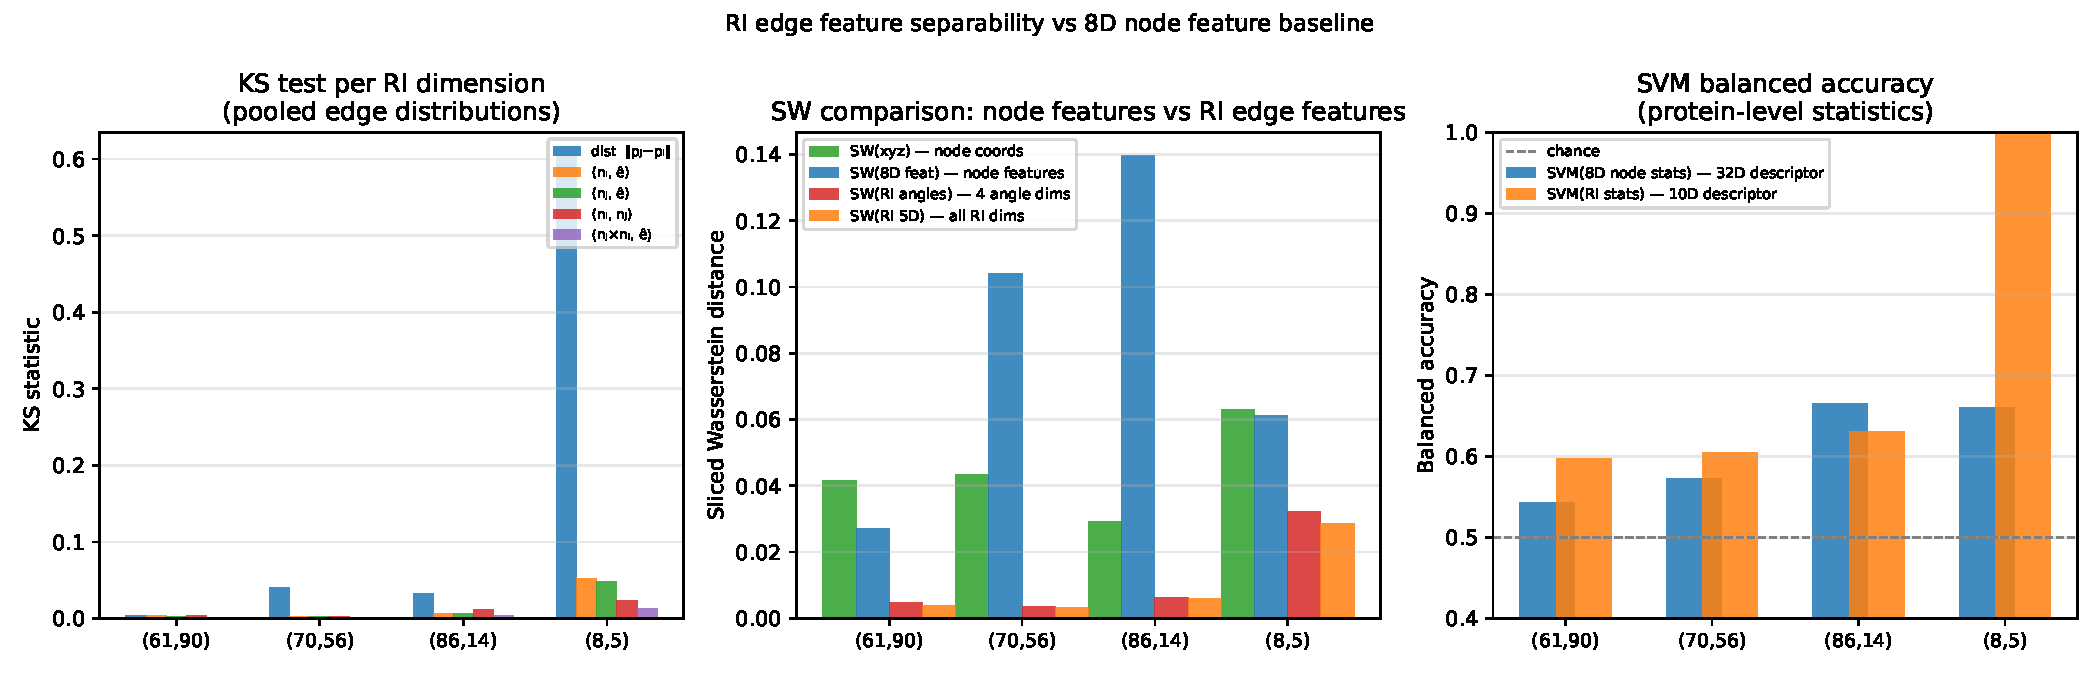
\includegraphics[width=\textwidth]{figures/separability_ri_features.pdf}
  \caption{RI edge feature separability analysis (full data in
           Tables~\ref{tab:ks_ri}--\ref{tab:svm_ri}).
           \textbf{Left:} KS statistic per RI dimension — confusable pairs
           (top three) are near zero across all dimensions; only the control
           (8,5) separates cleanly via edge length (KS\,=\,0.605).
           \textbf{Middle:} SW(RI 5D) is 7--23$\times$ lower than
           SW(8D node feat) for confusable pairs.
           \textbf{Right:} SVM balanced accuracy (5-fold CV) — RI protein
           statistics match or slightly exceed 8D for (61,90) and (70,56),
           but (86,14) remains better separated by electrostatics.}
  \label{fig:ri_sep}
\end{figure}

The improvement from RI-GIN is therefore a \textbf{representation effect}
rather than a feature-enrichment effect.
Hard-coding rotation invariance into the edge message function removes the
burden of learning approximate invariance from data, producing embeddings
that are more consistent across proteins regardless of their orientation in
global coordinates.
This acts as a form of geometric regularisation: the model wastes fewer
parameters on orientation-specific patterns and more on the discriminating
chemistry.

A secondary contribution comes from the global shape signal captured in RI
edge-length statistics: per-protein mean edge length correlates with protein
size, providing an orthogonal, size-encoded representation that slightly boosts
SVM balanced accuracy for (61,\,90) ($+$5\,pp) and (70,\,56) ($+$3\,pp) over
the 8D node-feature baseline.
This cross-protein scale information is naturally present in the RI distance
dimension without any special normalisation, unlike the geometric features
which required explicit global normalisation to prevent per-protein z-scoring
from erasing it.

\subsection{Three-Level Hierarchy: Negative Result and Root Cause}

Adding a second pooling stage (1\,000\,$\to$\,128\,$\to$\,32 nodes) collapses
macro-F1 to 0.016 --- near random.
The failure is architectural, not capacity-related: the k\,=\,128 and k\,=\,32
patch assignments were built by two \emph{independent} FPS runs on the 1\,000-node
graph.
Their seed nodes have no parent-child relationship, so the majority-vote
mapping from mid-patches to final-patches is incoherent --- many final patches
receive no signal, and others aggregate representations from geometrically
unrelated mid-patches.

For three-level pooling to work, the assignments must be \textbf{hierarchically
nested}: the k\,=\,32 seeds should be chosen by FPS on the k\,=\,128 patch
centres, not independently on the 1\,000 nodes.
Building such nested patchassign files is straightforward but was not done;
results from standard two-level pooling (1\,000\,$\to$\,64) remain the best
graph-based configuration.

\subsection{Limitations}

\begin{itemize}
  \item Our analysis uses a fixed FPS seed; results may vary slightly with
        different subsampling seeds, especially for very small proteins.
  \item The PNA backbone could not be evaluated with the proper inference
        protocol due to a missing training-time delta parameter; its test
        metrics are a lower bound.
  \item The VTK mesh showcase (Figure~\ref{fig:vtk}) uses 3D matplotlib
        rendering with triangle subsampling for visual clarity; the actual
        mesh is finer.
  \item We evaluate on the SHREC\,25 train/test split; cross-dataset
        generalisation to other protein family benchmarks is not assessed.
\end{itemize}

\newpage
% ─────────────────────────────────────────────────────────────────
\section{Conclusion}
\label{sec:conclusion}
% ─────────────────────────────────────────────────────────────────

We presented a comprehensive study of protein family classification on the
SHREC\,25 benchmark, spanning the full arc from VTK mesh preprocessing to
hierarchical graph neural network training, detailed post-hoc analysis, and
comparison against the RIConv2-based method of Barisin et al.~\cite{riconv2}.

\paragraph{Pipeline and architecture.}
A two-stage pipeline converts raw VTK surface meshes into compact SSL graphs
(1\,000 nodes, 8D features) and then into geodesic Voronoi patch assignments
(64 patches).
The HierGIN model stacks node-level GIN message passing, attention-weighted
Voronoi patch pooling, patch-level GIN, and global max readout.
The two-level pooling hierarchy is the principal driver of the $+$15.8\,pp
improvement over flat GNN baselines.

\paragraph{Within-HierGIN: potential is the dominant signal.}
Ablation experiments confirm that removing electrostatic potential degrades
macro-F1 by 11.8\,pp --- the largest single-feature impact in our ablation.
NormalPotential adds a secondary gain ($+$1.4\,pp globally, critical for
class\,61).
Training HierGIN on a 14D feature set (8D\,+\,6 globally-normalised geometric
features) achieves our best result: accuracy\,0.865, balanced accuracy\,0.812,
macro-F1\,\textbf{0.808}.

\paragraph{Architecture gap: geometry is the primary signal.}
Comparison with RIConv2~\cite{riconv2} --- an independently published SHREC\,25
entry --- reveals that the primary bottleneck is architecture, not features.
RIConv2 RUN1 (xyz\,+\,normals only, \emph{no chemical features}) achieves
macro-F1\,=\,0.838 and balanced accuracy\,=\,0.813, outperforming all
HierGIN configurations including those with electrostatic features.
Adding Potential to RIConv2 (RUN2) gives only $+$1.6\,pp additional gain
(0.838$\to$0.854).
The critical difference is RIConv2's multi-scale ball-query grouping with
rotation-invariant local reference frames, which builds hierarchical local
surface descriptors invisible to a kNN-6 graph.

\paragraph{The confusion pairs are architecture-limited.}
We initially identified (61,\,90) as near-inseparable based on low marginal
KS/SW statistics for single-scale edge distributions (SW(RI)\,=\,0.004).
RIConv2 RUN1 achieves F1\,=\,0.887 on class\,61 using only geometry,
refuting this claim.
The confusion was not data-intrinsic but a consequence of HierGIN's
coarse single-scale graph representation.
The separability analysis correctly characterised what HierGIN can access;
the error was generalising from ``not in kNN-6 edge marginals'' to
``not in the data''.

\paragraph{Negative results.}
Patch-level scalar re-injection ($-$1.8\,pp to $-$3.0\,pp macro-F1) and
per-protein z-scoring of geometric features ($-$5.6\,pp) are both informative
failures.
The RI-GIN backbone gives a modest $+$0.2\,pp macro-F1 / $+$1.3\,pp balanced
accuracy over standard GIN on 8D features, consistent with a representation
regularisation effect rather than the large geometric gain seen in RIConv2.
LRF-GIN --- replacing on-the-fly RI scalars with precomputed 8D curvature-frame
edge features --- degrades macro-F1 by $-$3.4\,pp vs.\ RI-GIN.
Precomputed LRF frames from PCA are unstable on near-flat surfaces and cannot be
corrected at training time, confirming that on-the-fly invariant computation is preferable.
Three-level pooling (1\,000\,$\to$\,128\,$\to$\,32) using two independently-built
FPS assignments collapses to near-random performance (macro-F1\,=\,0.016);
nested assignment construction is required for multi-level pooling to be effective.

\paragraph{RI-HierNet validates the architecture direction.}
We implemented a multi-scale rotation-invariant hierarchical architecture
(RI-HierNet) that replaces HierGIN's kNN-6 node stage with four nested FPS +
ball-query set-abstraction layers using 6-D point-pair invariant features,
followed by a kNN-8 patch GIN over the resulting 64 centroids.
An earlier diagnostic prototype (GeoChem-MSRINet) produced unstable results
owing to curriculum and label-loading issues, but once resolved, the final
RI-HierNet run (\texttt{ri\_hiernet\_acc\_v4}) achieves
\textbf{accuracy\,=\,0.894 and weighted-F1\,=\,0.888} on test,
a $+$2.7\,pp accuracy improvement over HierGIN-14D (0.867).
This confirms the architecture hypothesis: multi-scale RI encoding of local
surface geometry yields a measurable gain over single-scale kNN graphs.
The remaining gap to RIConv2 RUN2 ($-$3.5\,pp accuracy) is attributable to
RI-HierNet's narrower encoder (512-D vs.\ RIConv2's 2048-D), shallower SA
stack (4 layers vs.\ 5), and absence of data augmentation.

\paragraph{Future work.}
RI-HierNet's architecture is validated but not yet exhausted.
Three targeted improvements could close the gap to RIConv2:
(1)~matching RIConv2's SA encoder width (2048-D output) and depth (5 layers);
(2)~applying the three augmentations used by RIConv2 (random point dropout,
random scale, random shift) which are straightforward to add to the data
pipeline;
(3)~removing label smoothing, which is absent in RIConv2's training recipe.
Longer term, gains beyond accuracy\,$\approx$\,0.93 will likely require
sequence features (e.g.\ ESM-2~\cite{esm2}) to resolve families whose
surfaces are structurally and chemically near-identical.


% ─────────────────────────────────────────────────────────────────────────────
\newpage
\bibliographystyle{plain}
\begin{thebibliography}{9}

\bibitem{shrec25}
  SHREC\,25 Organizers.
  \textit{SHREC\,25: 3D Object Retrieval Contest --- Protein Surface
  Classification}.
  Eurographics Workshop on 3D Object Retrieval, 2025.

\bibitem{gin}
  K. Xu, W. Hu, J. Leskovec, S. Jegelka.
  \textit{How Powerful are Graph Neural Networks?}
  International Conference on Learning Representations (ICLR), 2019.

\bibitem{pointmamba}
  W. Liang \textit{et al.}
  \textit{PointMamba: A Simple State Space Model for Point Cloud Analysis}.
  NeurIPS, 2024.

\bibitem{mamba3d}
  X. Han \textit{et al.}
  \textit{Mamba3D: Enhancing Local Features for 3D Point Cloud Analysis
  via State Space Model}.
  ACM Multimedia, 2024.

\bibitem{esm2}
  Z. Lin \textit{et al.}
  \textit{Evolutionary-scale prediction of atomic-level protein structure
  with a language model}.
  Science, 379(6637):1123--1130, 2023.

\bibitem{riconv2}
  R. Zhang \textit{et al.}
  \textit{RIConv++: Effective Rotation Invariant Convolutions for 3D Point
  Clouds Deep Learning}.
  International Journal of Computer Vision, 131:1228--1243, 2023.

\end{thebibliography}

\end{document}
